\begin{center}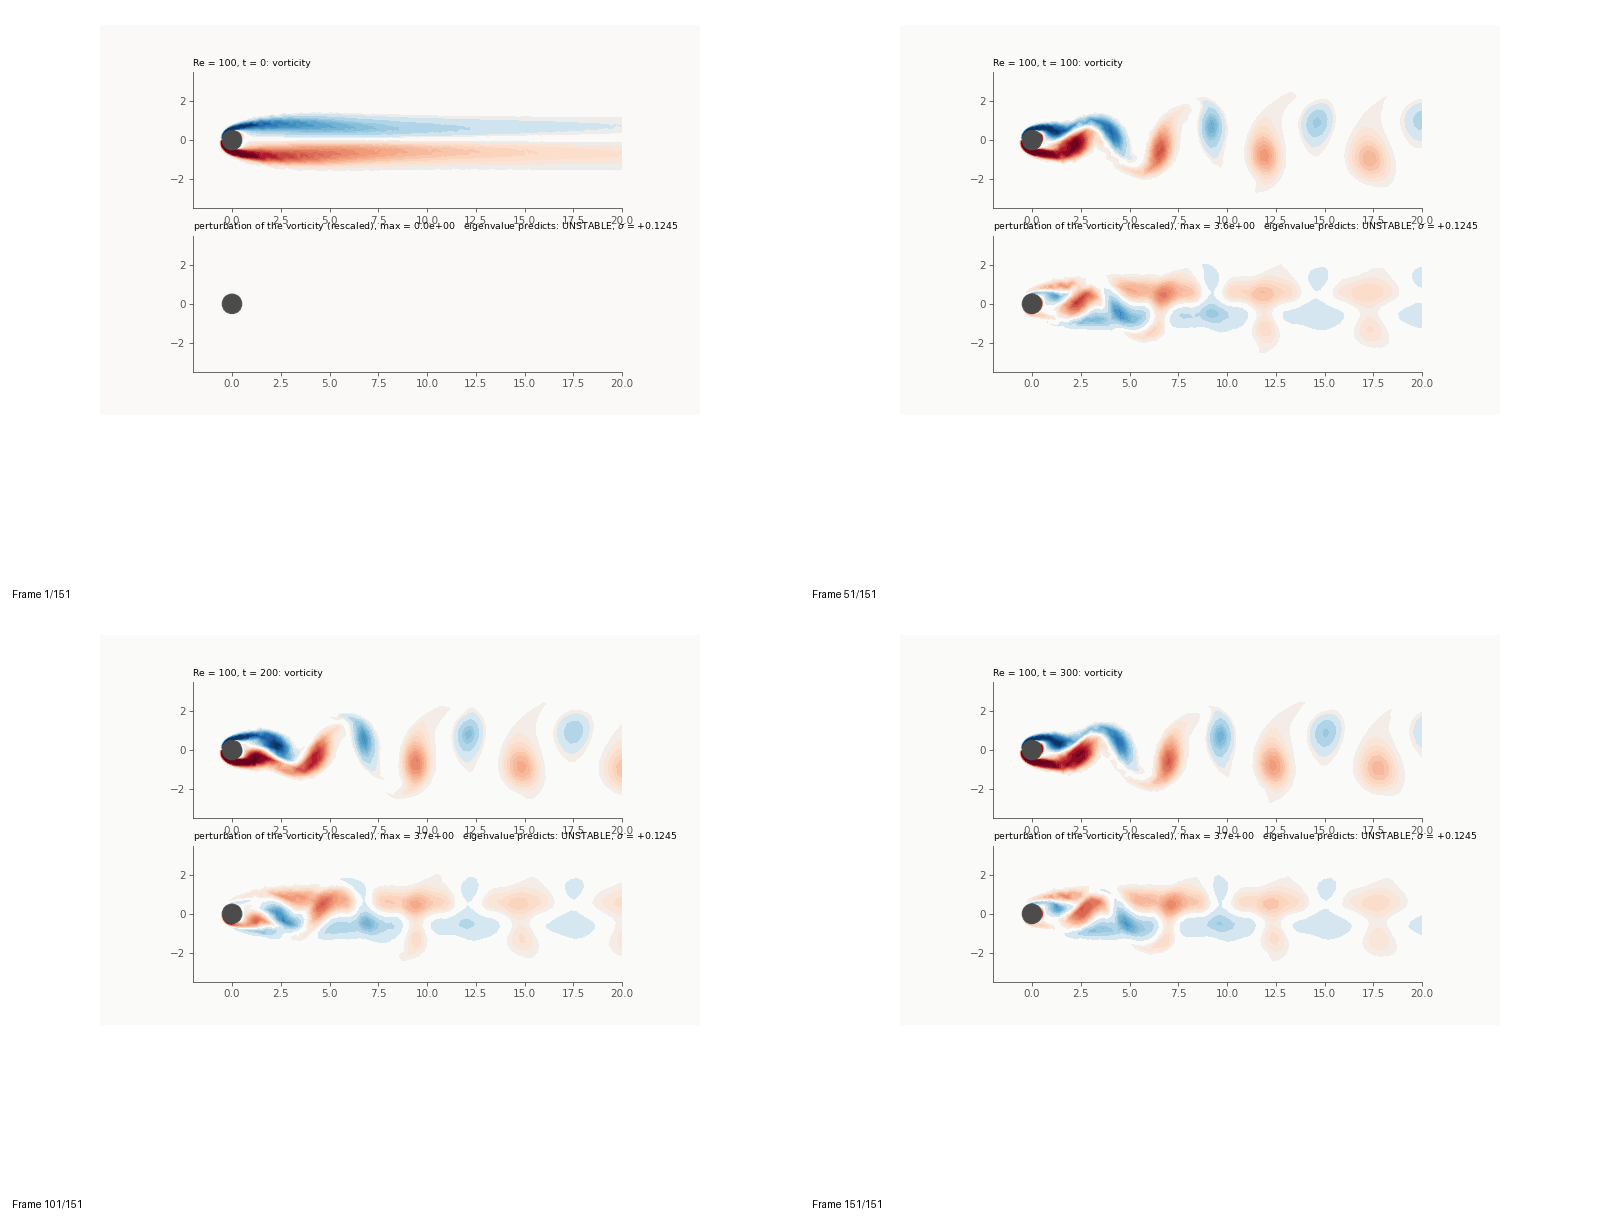
\includegraphics[width=\linewidth,height=170mm,keepaspectratio]{animation_stills/wake_dns_Re100_vorticity.png}\captionof{figure}[Archived figure]{Cylinder benchmark at Reynolds number one hundred: nonlinear saturated vortex shedding. Four ordered frames are selected by frame index; spacing is not asserted to be uniform in physical time. \textit{Original GIF:} \path{research/Navier_Stokes_Inflow/stability/figures/dns_Re100_vorticity.gif}. First added 2026-09-29.}\end{center}
\noindent\textit{Playback file in this source package:} \path{figures/wake_dns_Re100_vorticity.gif}.\clearpage
\begin{center}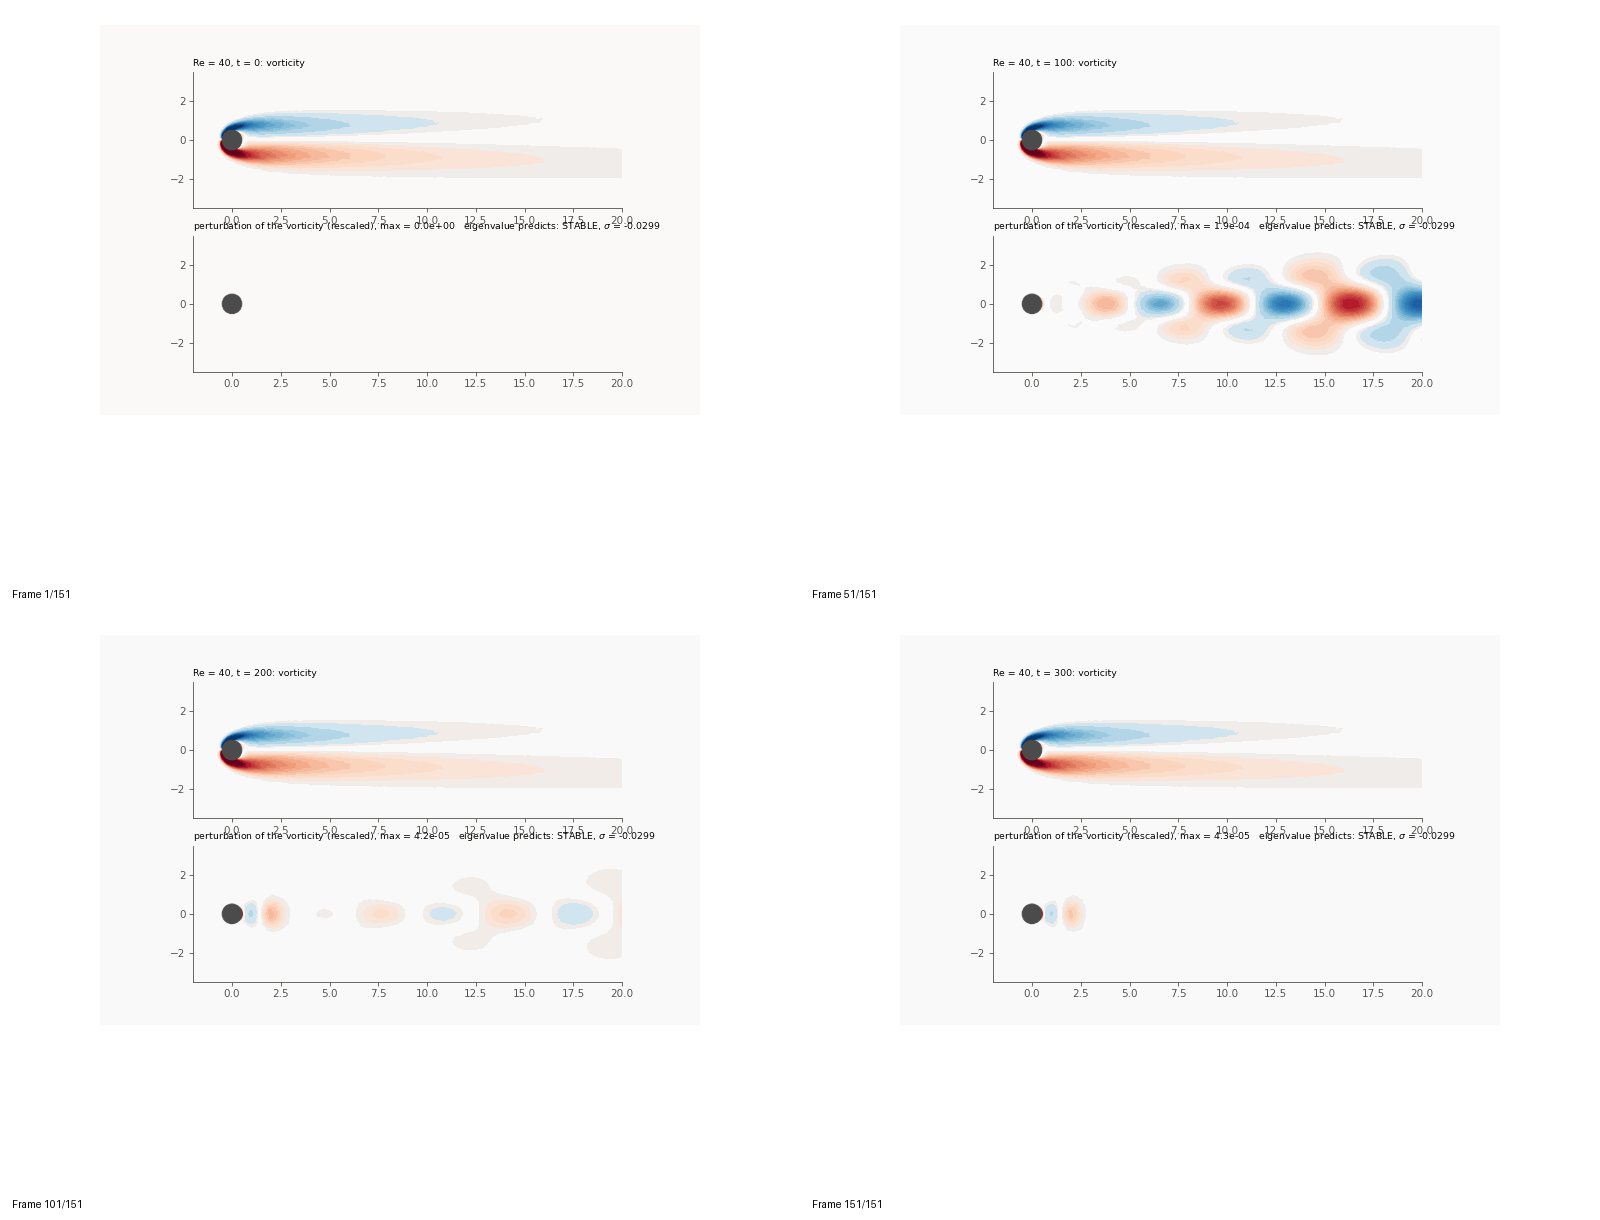
\includegraphics[width=\linewidth,height=170mm,keepaspectratio]{animation_stills/wake_dns_Re40_vorticity.png}\captionof{figure}[Archived figure]{Cylinder benchmark below onset: an initial perturbation decays to a steady symmetric wake. Four ordered frames are selected by frame index; spacing is not asserted to be uniform in physical time. \textit{Original GIF:} \path{research/Navier_Stokes_Inflow/stability/figures/dns_Re40_vorticity.gif}. First added 2026-09-29.}\end{center}
\noindent\textit{Playback file in this source package:} \path{figures/wake_dns_Re40_vorticity.gif}.\clearpage
\begin{center}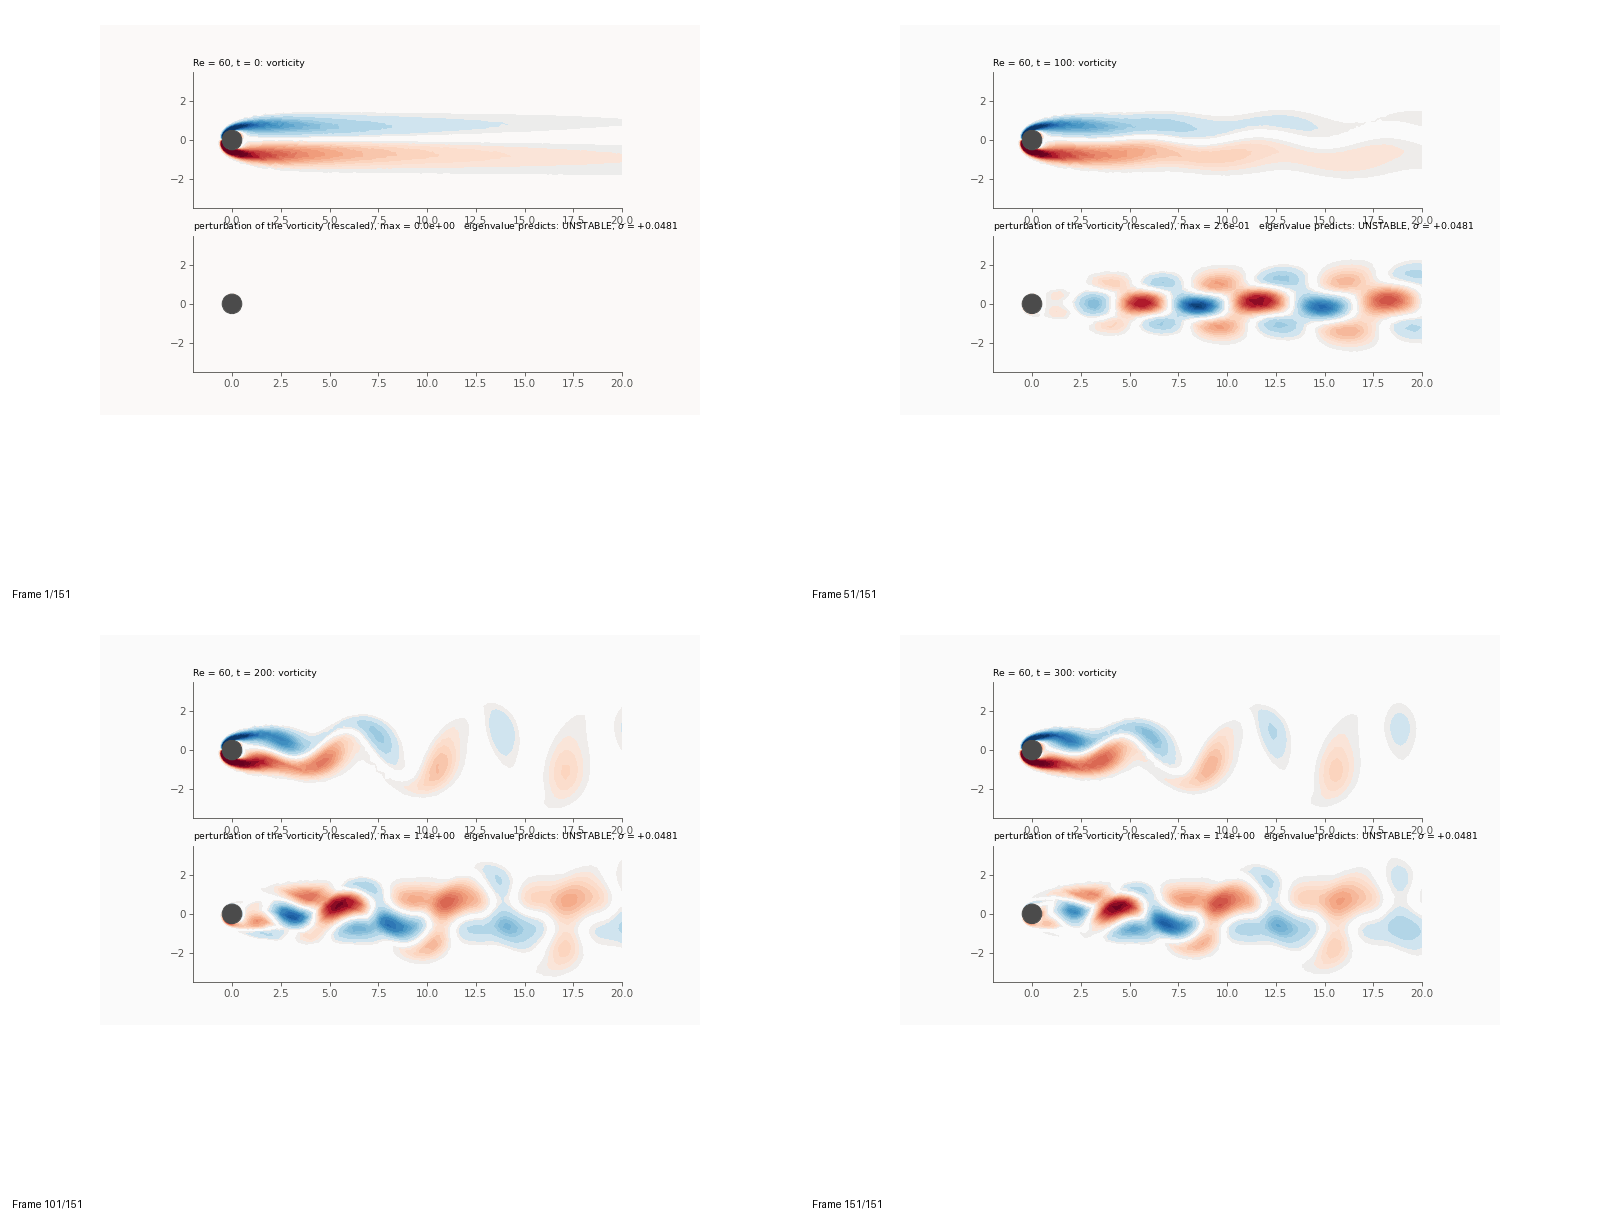
\includegraphics[width=\linewidth,height=170mm,keepaspectratio]{animation_stills/wake_dns_Re60_vorticity.png}\captionof{figure}[Archived figure]{Cylinder benchmark above onset: growing perturbations develop into a vortex street. Four ordered frames are selected by frame index; spacing is not asserted to be uniform in physical time. \textit{Original GIF:} \path{research/Navier_Stokes_Inflow/stability/figures/dns_Re60_vorticity.gif}. First added 2026-09-29.}\end{center}
\noindent\textit{Playback file in this source package:} \path{figures/wake_dns_Re60_vorticity.gif}.\clearpage
\begin{center}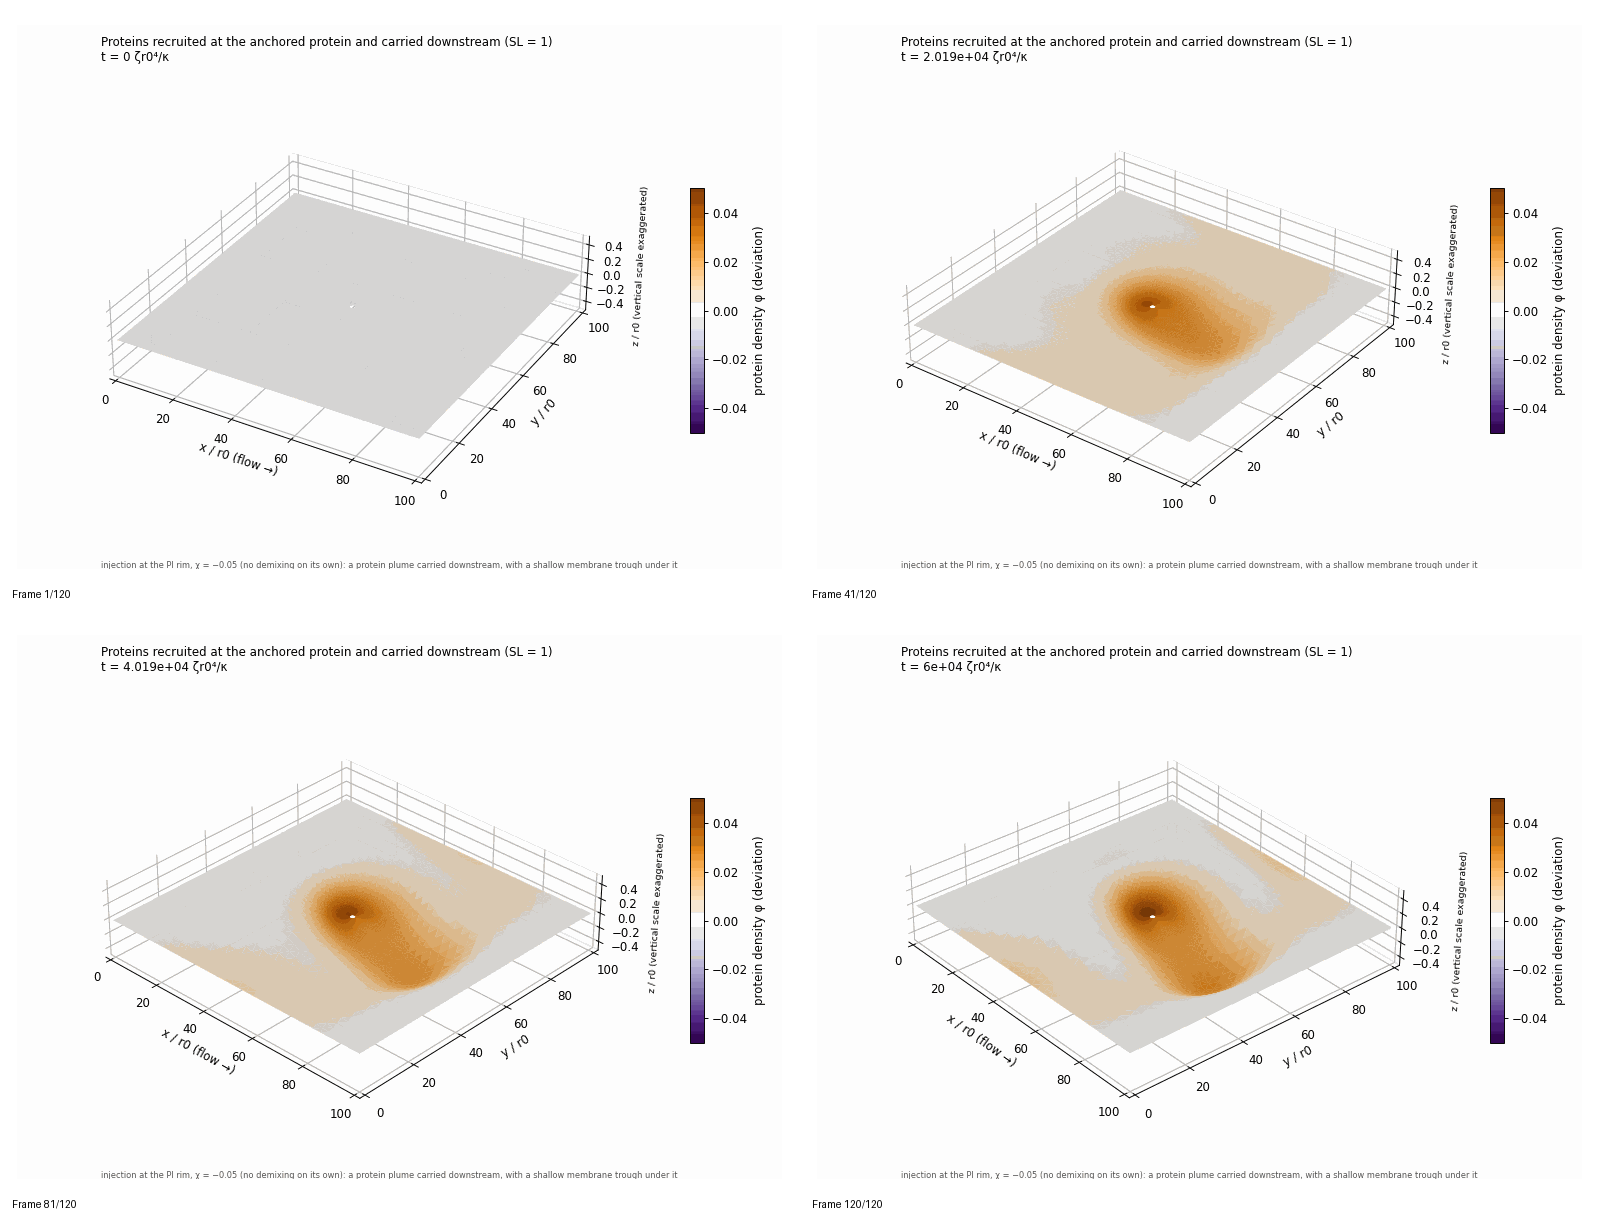
\includegraphics[width=\linewidth,height=170mm,keepaspectratio]{animation_stills/membrane_gif10_proteins_source_3d.png}\captionof{figure}[Archived figure]{Rim-source protein plume carried downstream with a shallow associated trough. The final run uses absorbing outflow. Four ordered frames are selected by frame index; spacing is not asserted to be uniform in physical time. \textit{Original GIF:} \path{research/membrane_stability/figures/gifs/gif10_proteins_source_3d.gif}. First added 2026-10-02.}\end{center}
\noindent\textit{Playback file in this source package:} \path{figures/membrane_gif10_proteins_source_3d.gif}.\clearpage
\begin{center}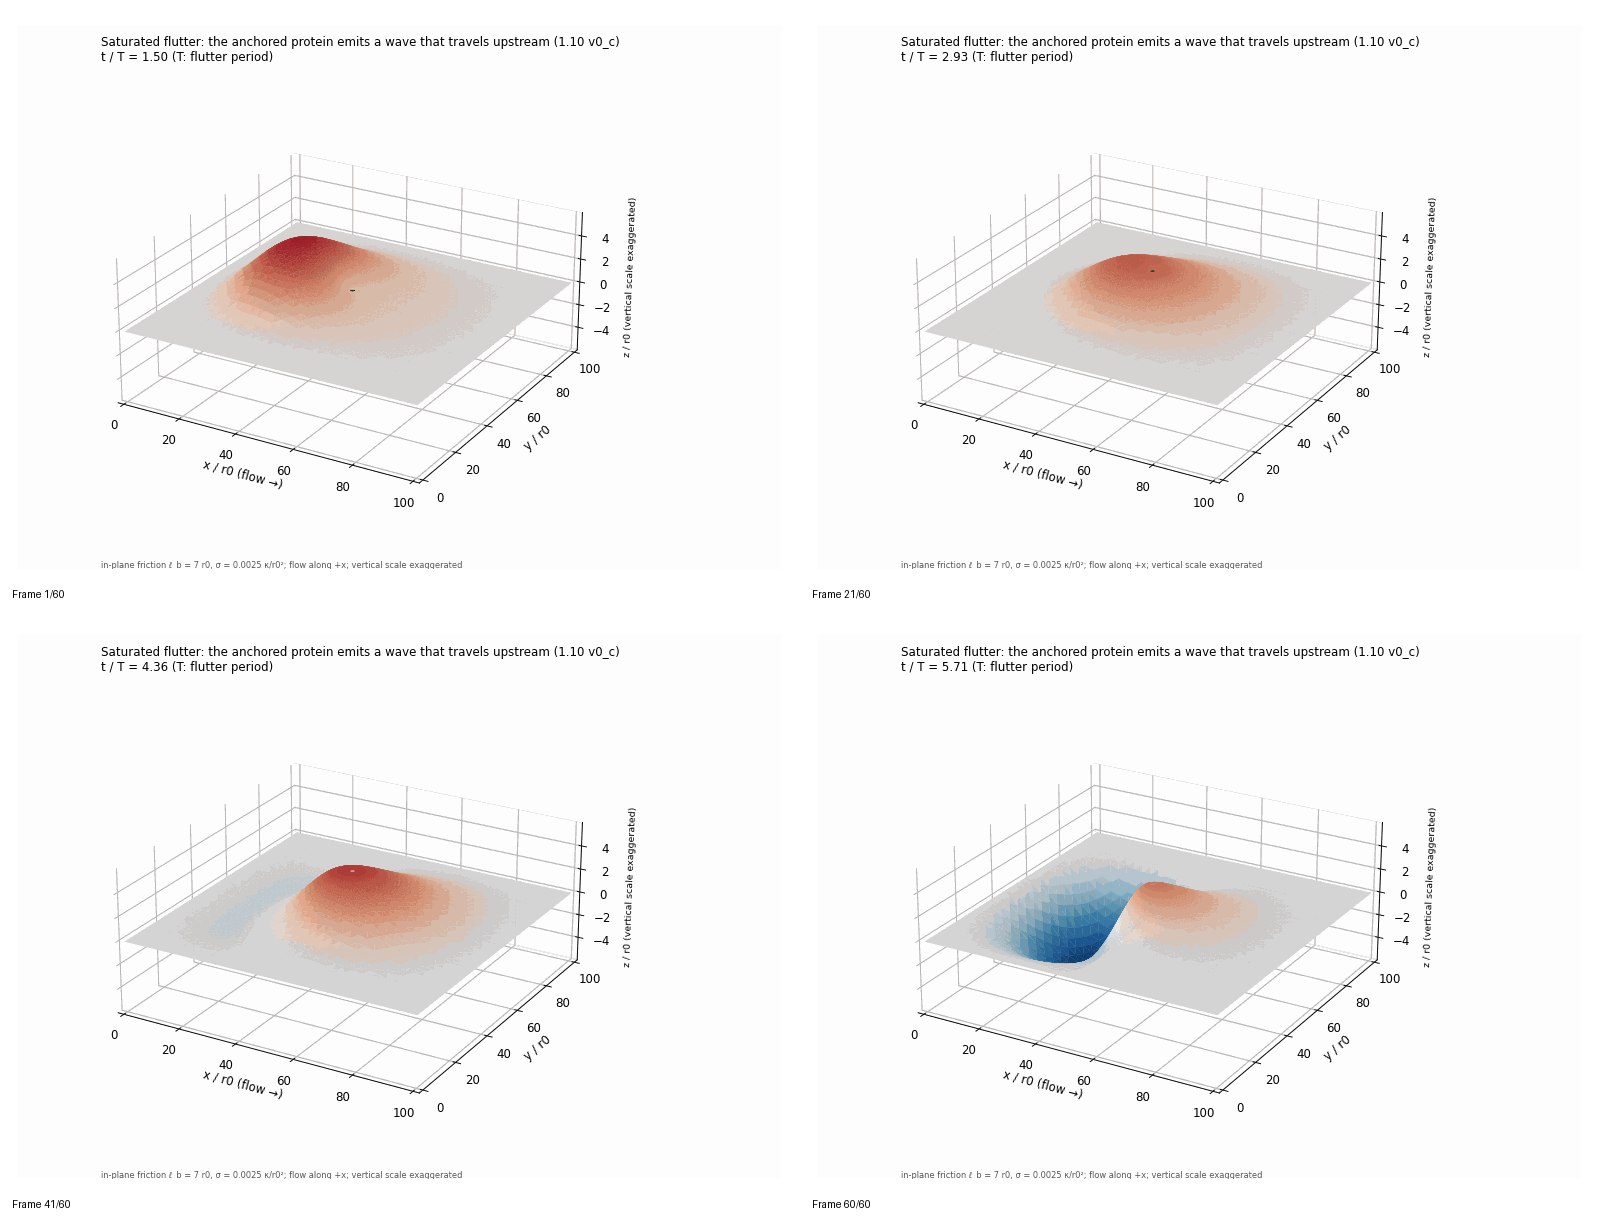
\includegraphics[width=\linewidth,height=170mm,keepaspectratio]{animation_stills/membrane_gif11_flutter_3d.png}\captionof{figure}[Archived figure]{Nonlinear friction-driven flutter: protein oscillation and a sustained source of upstream membrane waves. Four ordered frames are selected by frame index; spacing is not asserted to be uniform in physical time. \textit{Original GIF:} \path{research/membrane_stability/figures/gifs/gif11_flutter_3d.gif}. First added 2026-10-02.}\end{center}
\noindent\textit{Playback file in this source package:} \path{figures/membrane_gif11_flutter_3d.gif}.\clearpage
\begin{center}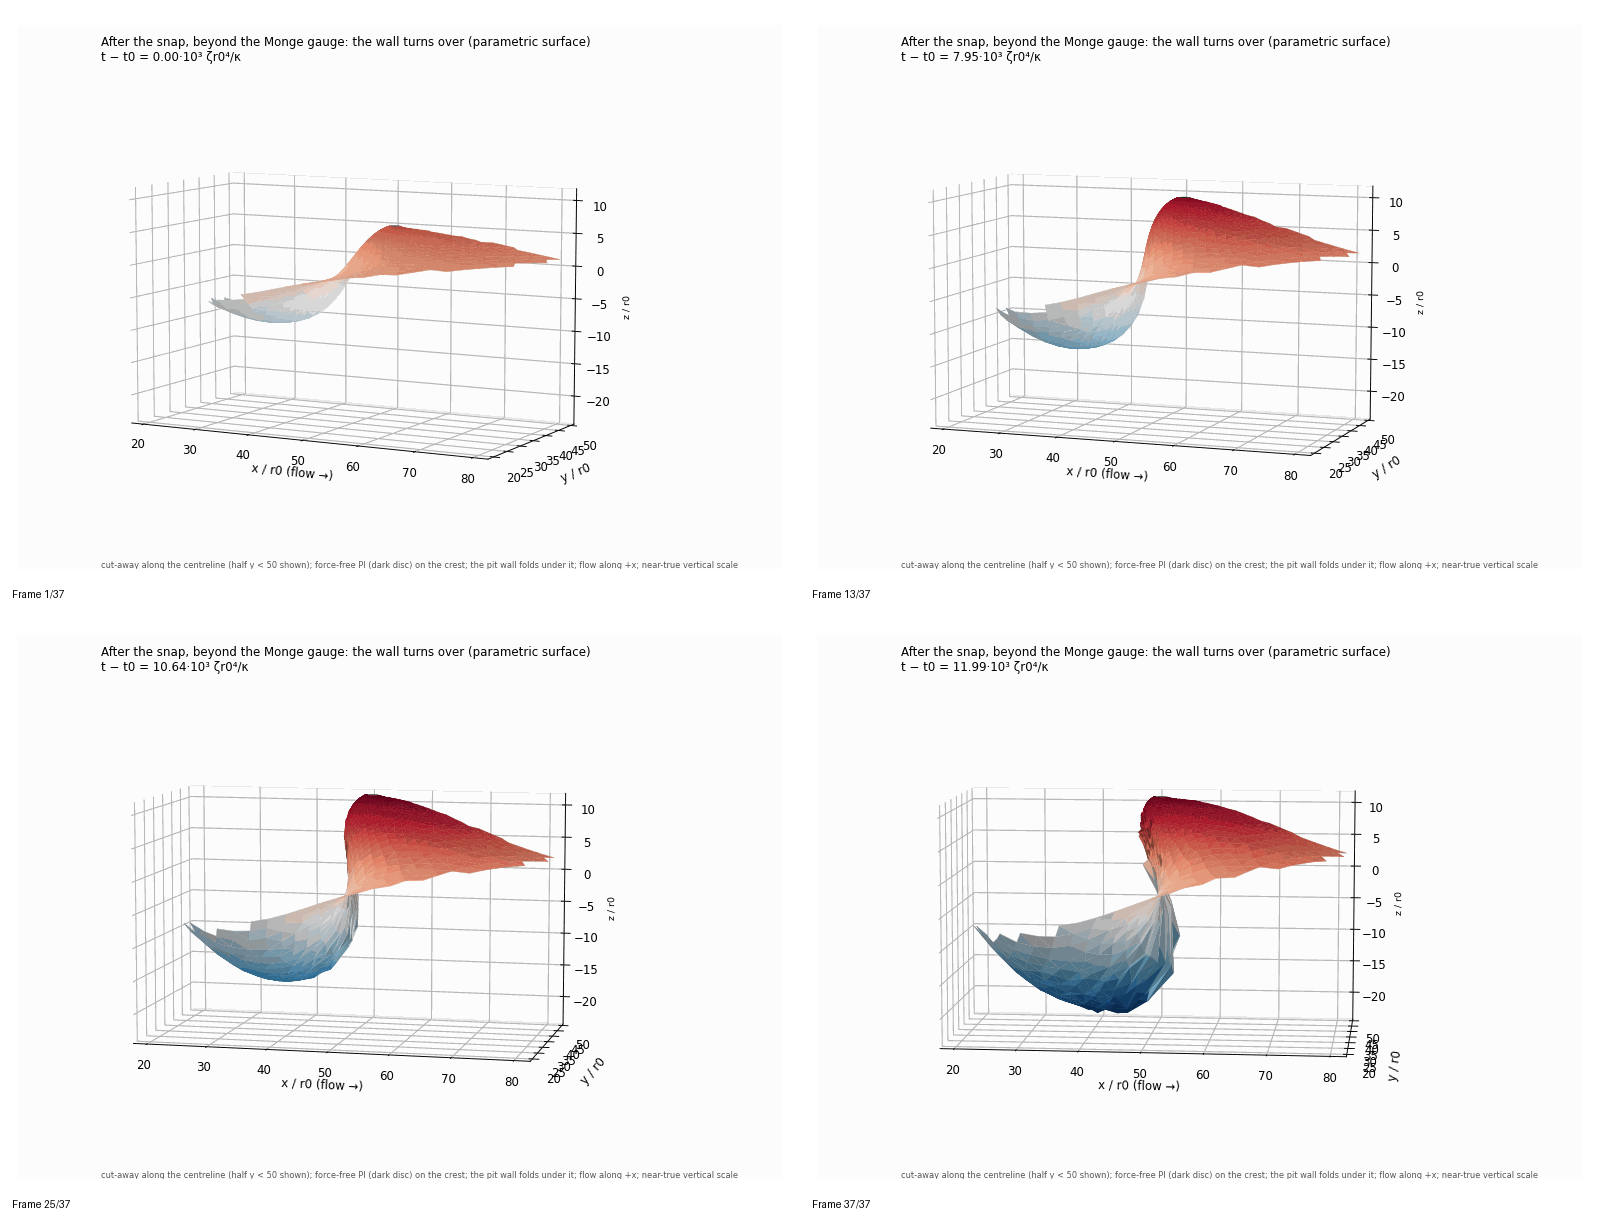
\includegraphics[width=\linewidth,height=170mm,keepaspectratio]{animation_stills/membrane_gif12_fold_parametric_3d.png}\captionof{figure}[Archived figure]{Parametric continuation of the force-free post-snap wall through vertical into an overhang underneath the lifted disc. The final state is distortion-limited. Four ordered frames are selected by frame index; spacing is not asserted to be uniform in physical time. \textit{Original GIF:} \path{research/membrane_stability/figures/gifs/gif12_fold_parametric_3d.gif}. First added 2026-10-02.}\end{center}
\noindent\textit{Playback file in this source package:} \path{figures/membrane_gif12_fold_parametric_3d.gif}.\clearpage
\begin{center}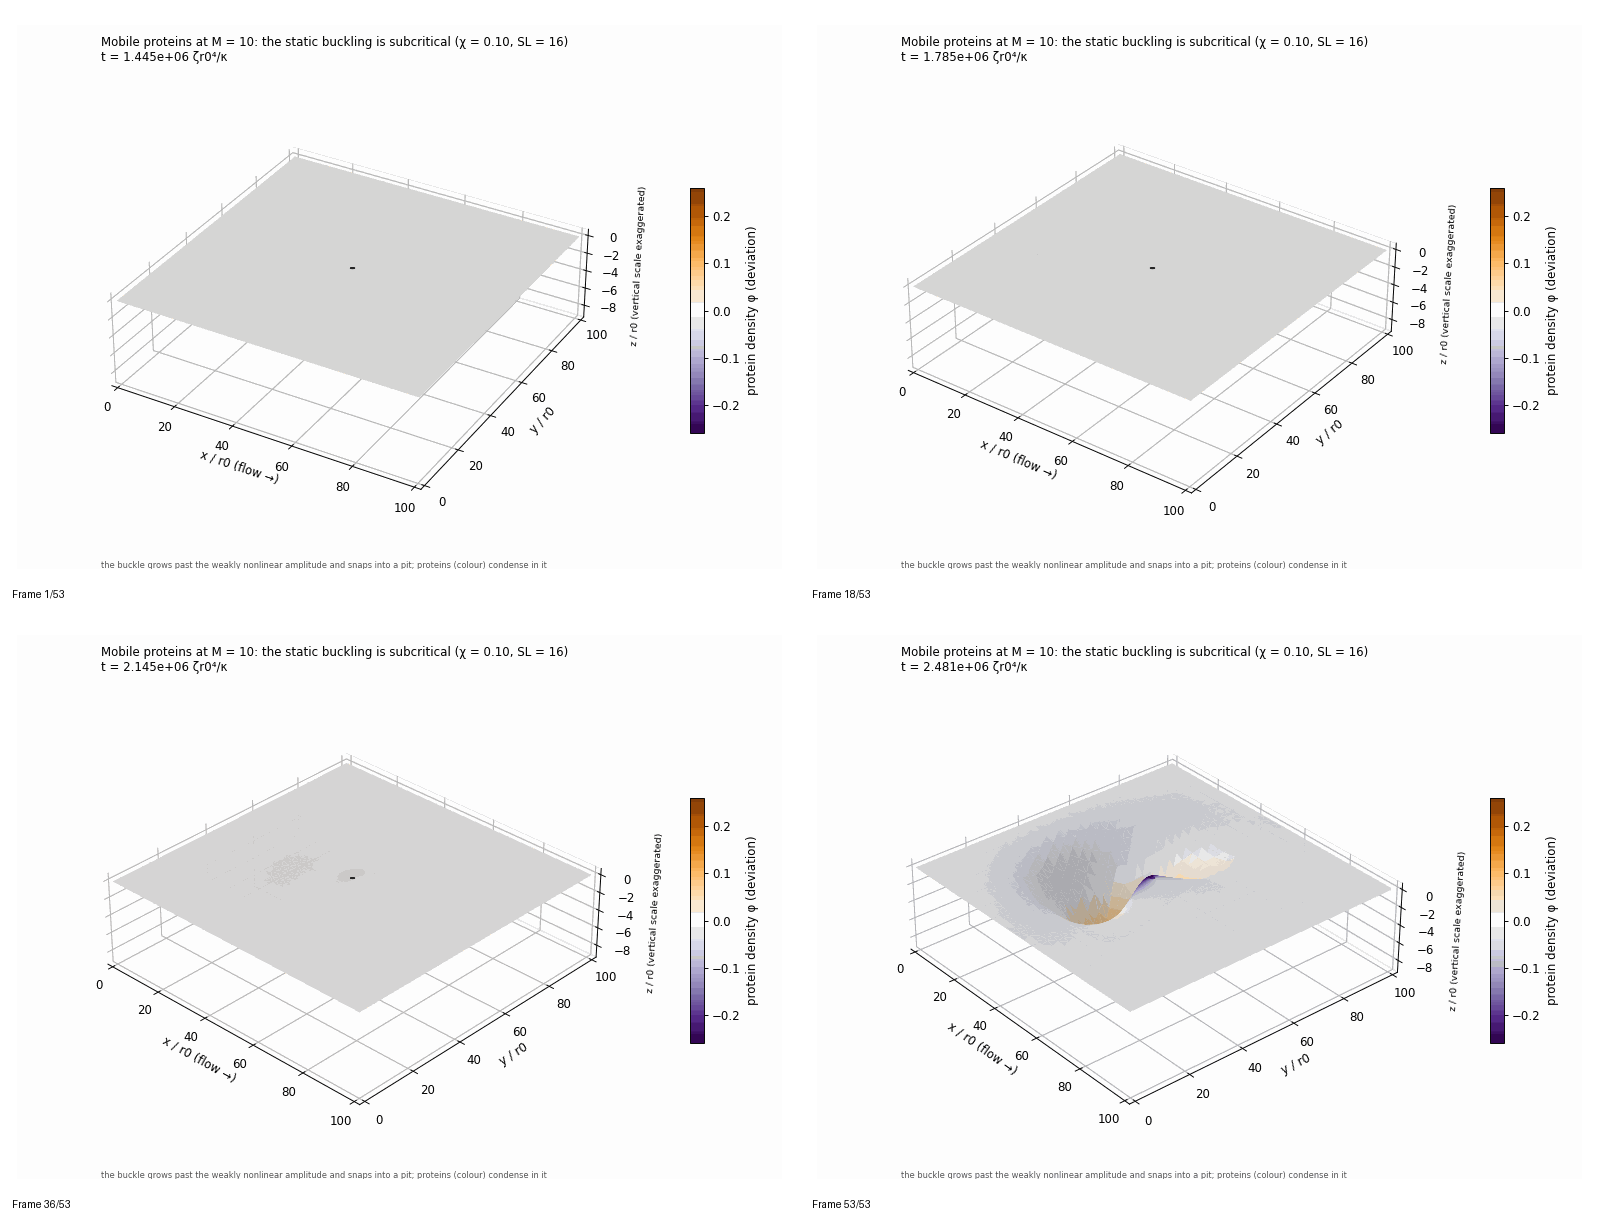
\includegraphics[width=\linewidth,height=170mm,keepaspectratio]{animation_stills/membrane_gif13_codim2_static_runaway_3d.png}\captionof{figure}[Archived figure]{Intermediate-mobility clamped-protein static-sector runaway. Shape and signed density deviation grow into a deep pit; no terminal attractor is resolved. Four ordered frames are selected by frame index; spacing is not asserted to be uniform in physical time. \textit{Original GIF:} \path{research/membrane_stability/figures/gifs/gif13_codim2_static_runaway_3d.gif}. First added 2026-10-03.}\end{center}
\noindent\textit{Playback file in this source package:} \path{figures/membrane_gif13_codim2_static_runaway_3d.gif}.\clearpage
\begin{center}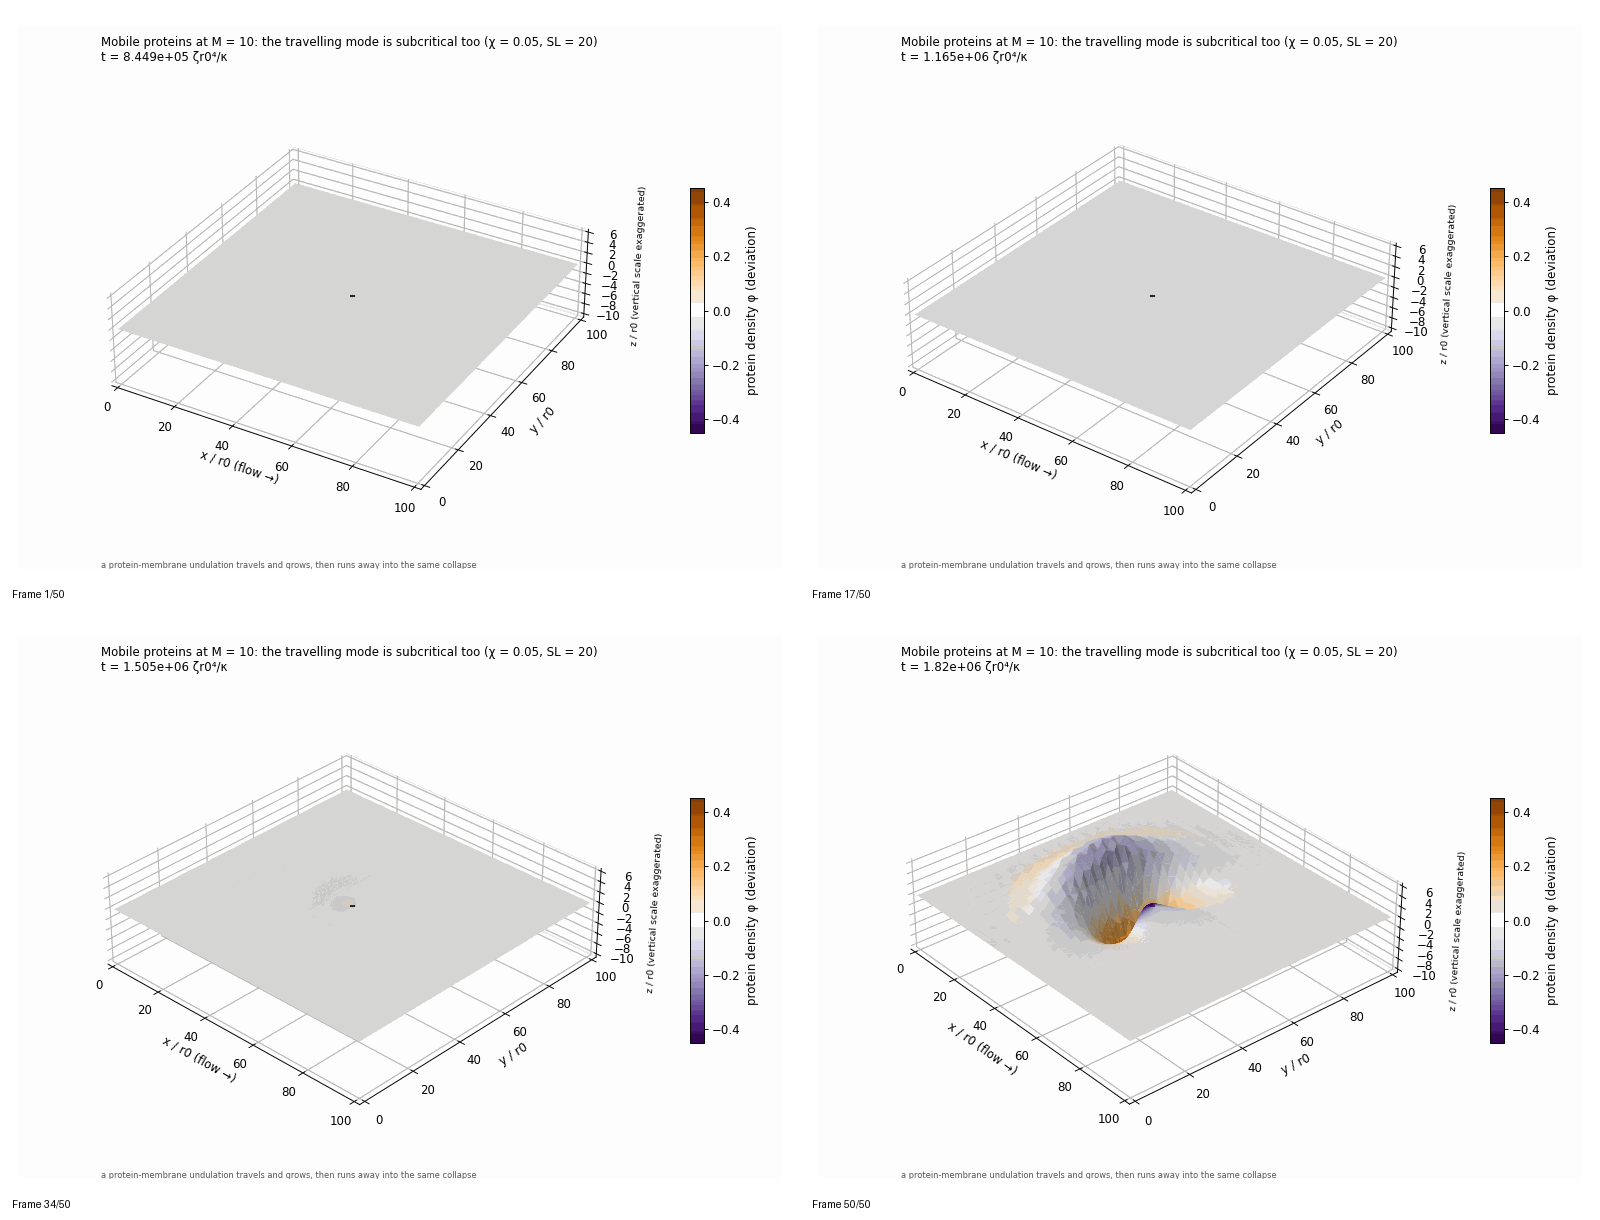
\includegraphics[width=\linewidth,height=170mm,keepaspectratio]{animation_stills/membrane_gif14_codim2_oscillatory_3d.png}\captionof{figure}[Archived figure]{Intermediate-mobility oscillatory-sector runaway. A growing travelling mode evolves into collapse rather than a saturated wave source. Four ordered frames are selected by frame index; spacing is not asserted to be uniform in physical time. \textit{Original GIF:} \path{research/membrane_stability/figures/gifs/gif14_codim2_oscillatory_3d.gif}. First added 2026-10-03.}\end{center}
\noindent\textit{Playback file in this source package:} \path{figures/membrane_gif14_codim2_oscillatory_3d.gif}.\clearpage
\begin{center}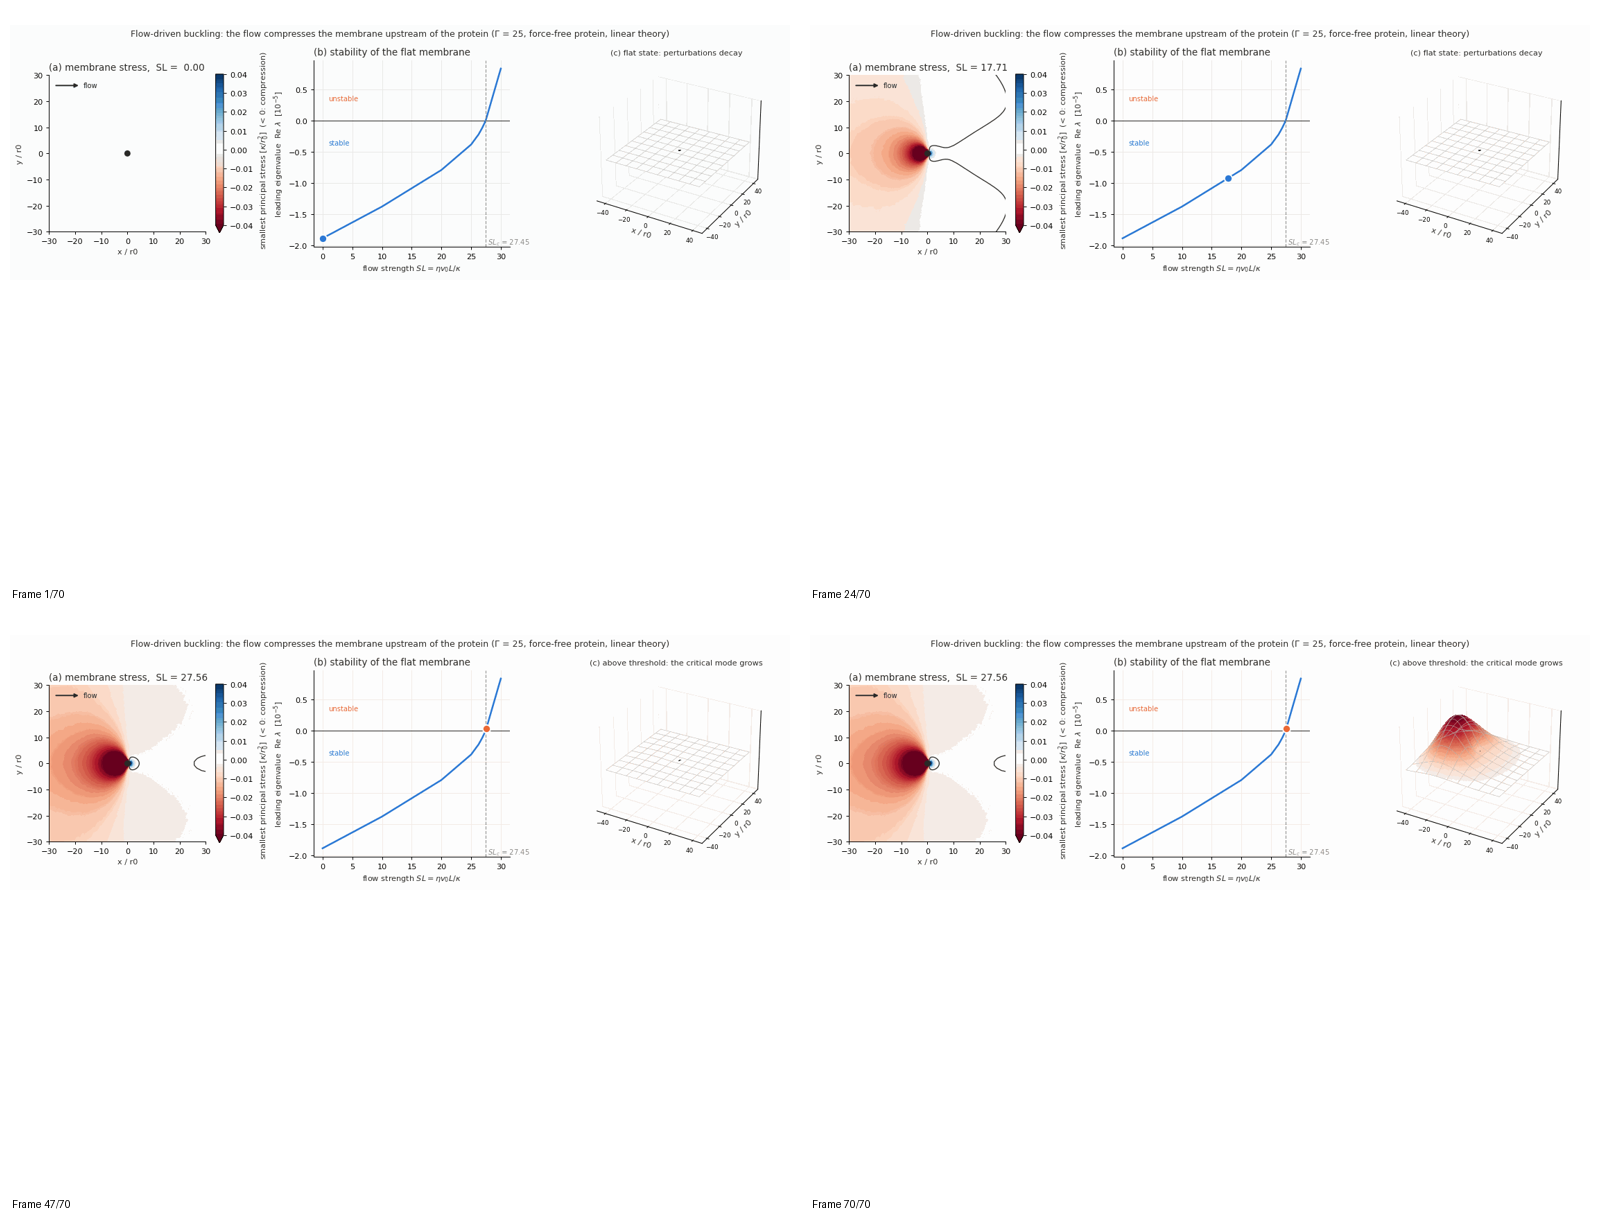
\includegraphics[width=\linewidth,height=170mm,keepaspectratio]{animation_stills/membrane_gif1_flow_buckling_onset.png}\captionof{figure}[Archived figure]{Critical-mode visualization of flow-driven buckling and upstream compression. This onset sequence belongs to the corrected study's visualization workflow; the static plots and force condition supply the quantitative threshold. Four ordered frames are selected by frame index; spacing is not asserted to be uniform in physical time. \textit{Original GIF:} \path{research/membrane_stability/figures/gifs/gif1_flow_buckling_onset.gif}. First added 2026-09-30.}\end{center}
\noindent\textit{Playback file in this source package:} \path{figures/membrane_gif1_flow_buckling_onset.gif}.\clearpage
\begin{center}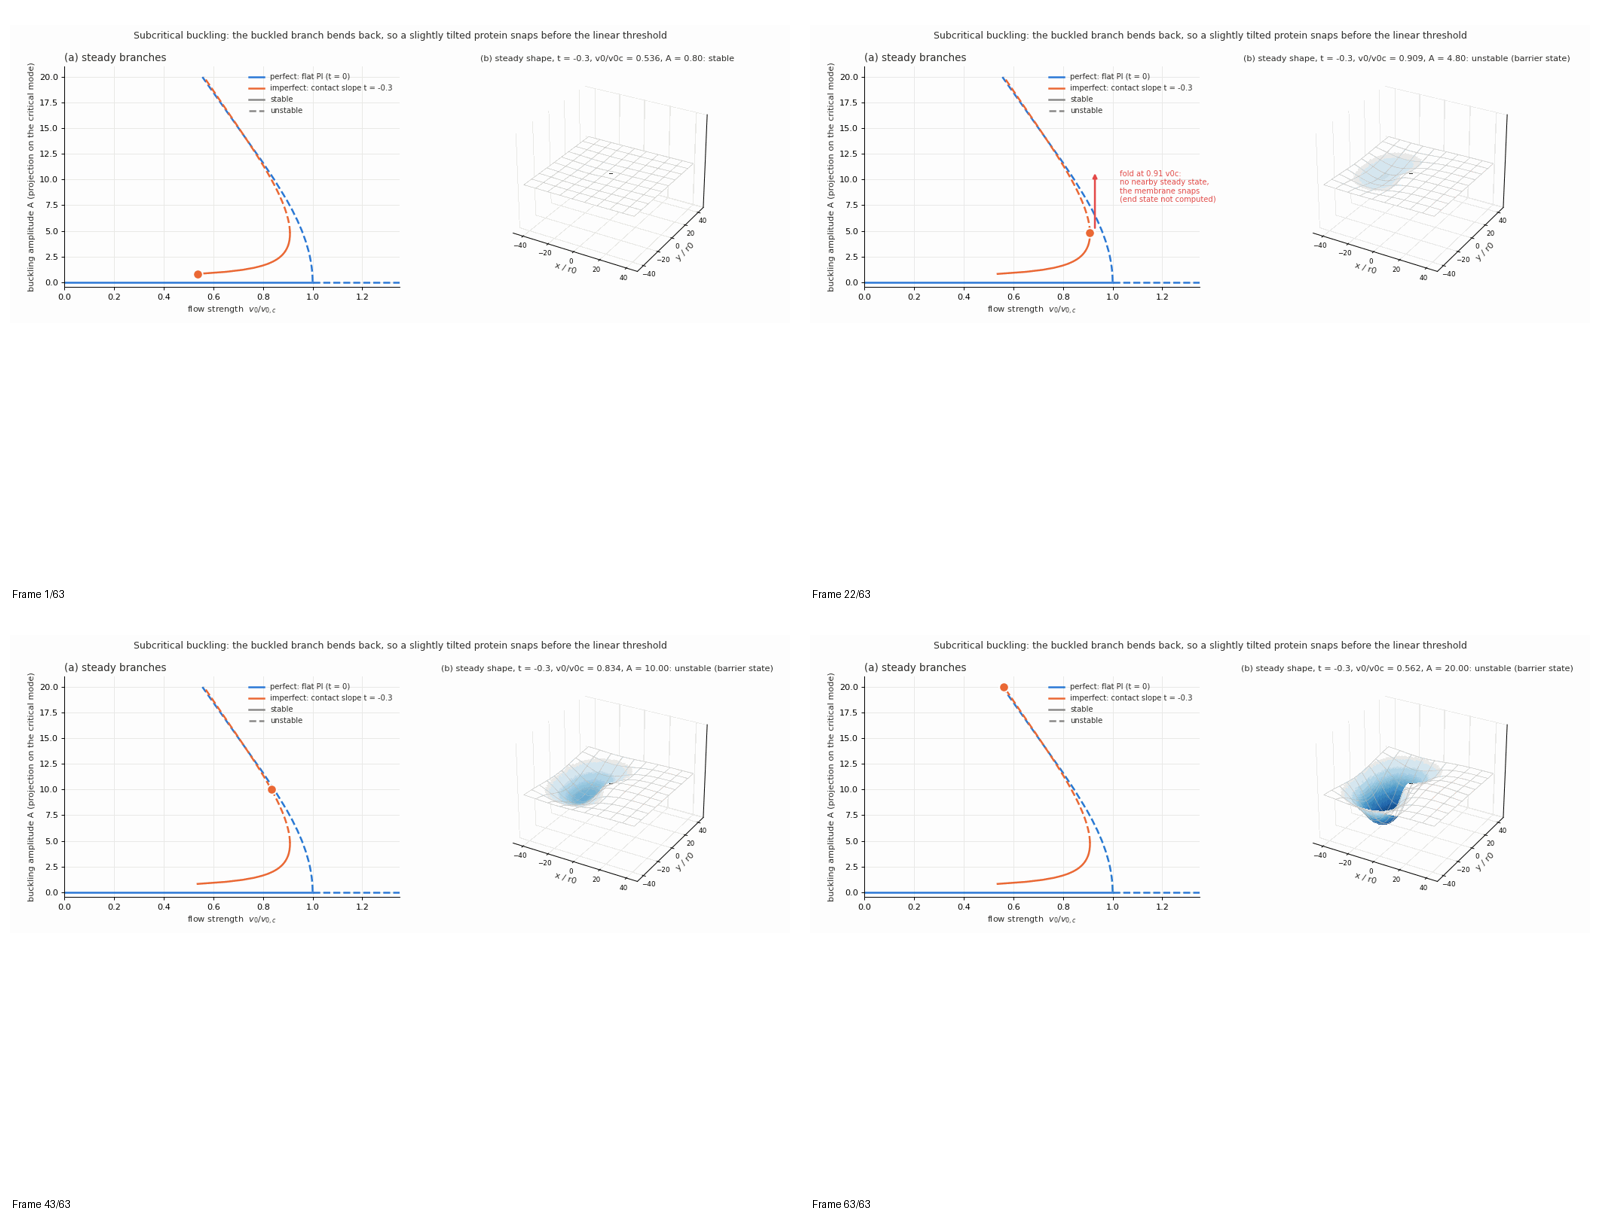
\includegraphics[width=\linewidth,height=170mm,keepaspectratio]{animation_stills/membrane_gif2_subcritical_snap.png}\captionof{figure}[Archived figure]{Branch visualization of the subcritical snap and its imperfection-sensitive fold. A continuation animation is a sequence of equilibria, not a physical-time simulation. Four ordered frames are selected by frame index; spacing is not asserted to be uniform in physical time. \textit{Original GIF:} \path{research/membrane_stability/figures/gifs/gif2_subcritical_snap.gif}. First added 2026-09-30.}\end{center}
\noindent\textit{Playback file in this source package:} \path{figures/membrane_gif2_subcritical_snap.gif}.\clearpage
\begin{center}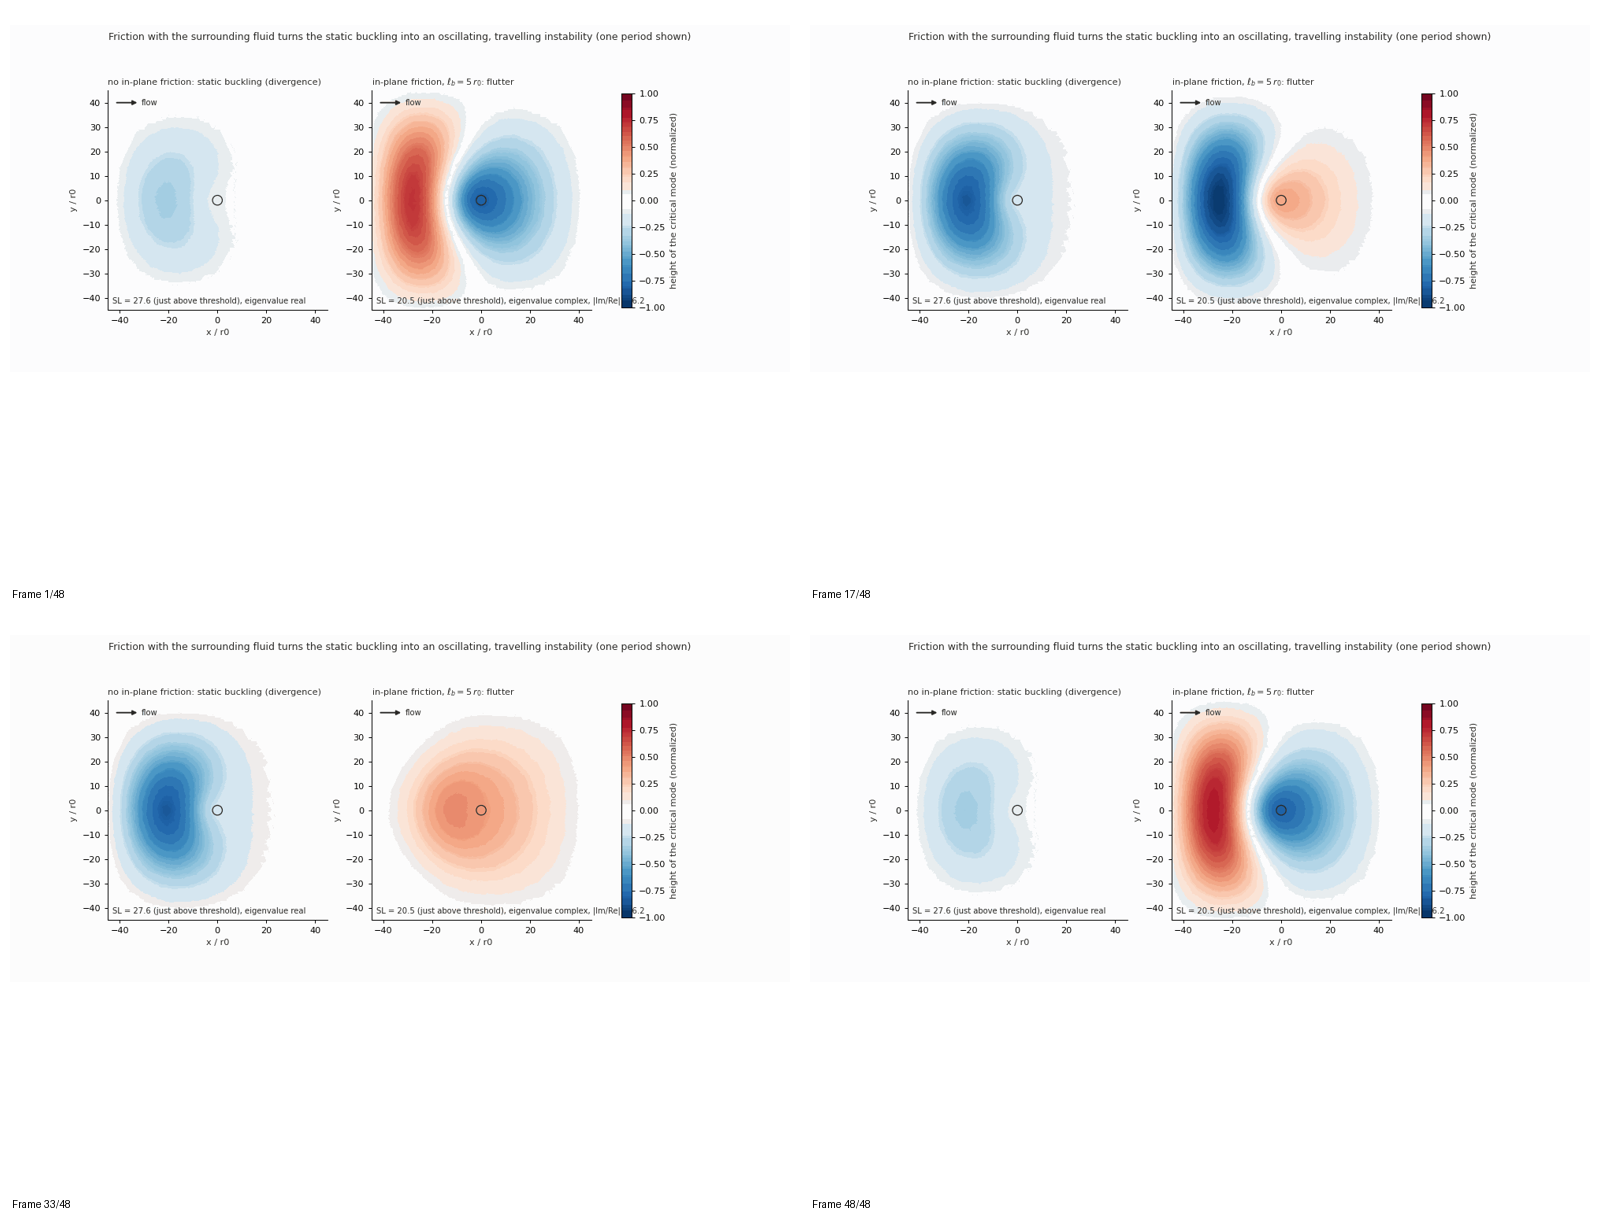
\includegraphics[width=\linewidth,height=170mm,keepaspectratio]{animation_stills/membrane_gif3_divergence_vs_flutter.png}\captionof{figure}[Archived figure]{Real divergence mode versus oscillatory flutter mode. The travelling phase of the complex mode is distinct from a nonlinear saturated cycle. Four ordered frames are selected by frame index; spacing is not asserted to be uniform in physical time. \textit{Original GIF:} \path{research/membrane_stability/figures/gifs/gif3_divergence_vs_flutter.gif}. First added 2026-09-30.}\end{center}
\noindent\textit{Playback file in this source package:} \path{figures/membrane_gif3_divergence_vs_flutter.gif}.\clearpage
\begin{center}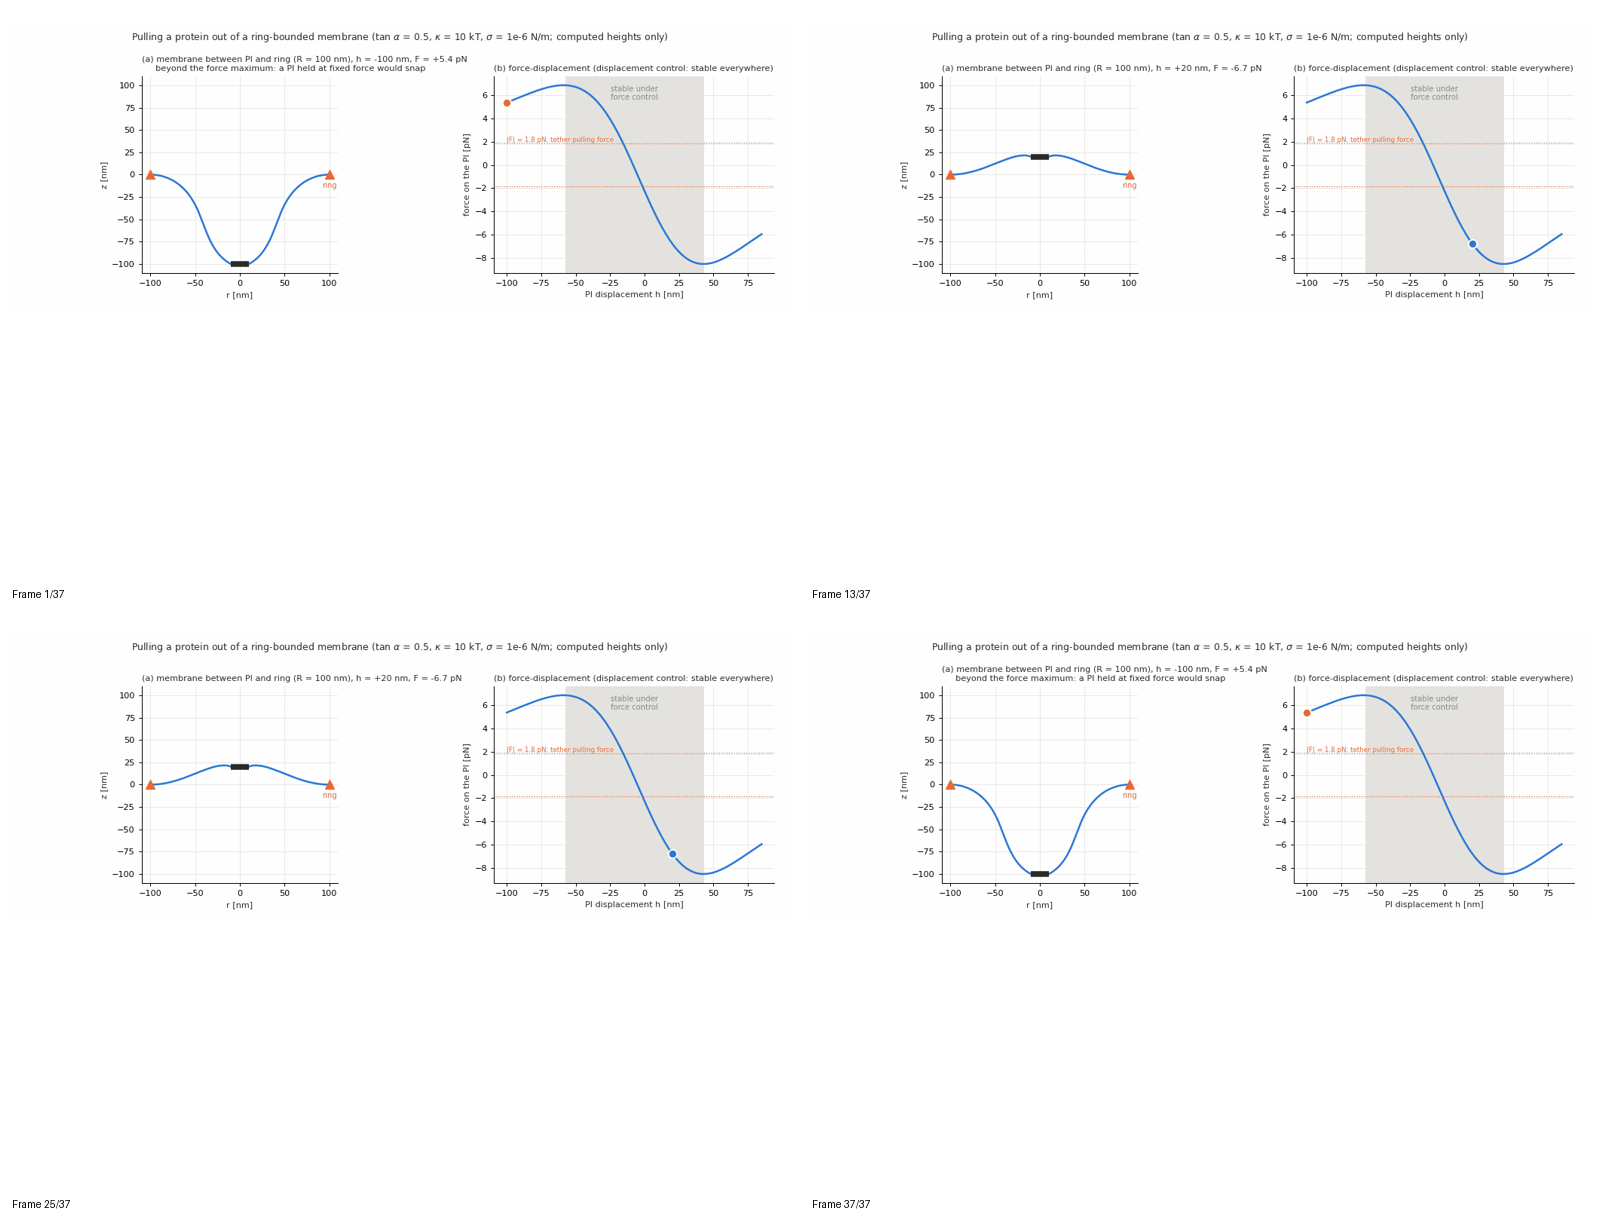
\includegraphics[width=\linewidth,height=170mm,keepaspectratio]{animation_stills/membrane_gif4_ring_pulling.png}\captionof{figure}[Archived figure]{Ring-pulling profile sequence. The imposed height varies along a branch; force-control stability is determined separately by the virtual-work stiffness. Four ordered frames are selected by frame index; spacing is not asserted to be uniform in physical time. \textit{Original GIF:} \path{research/membrane_stability/figures/gifs/gif4_ring_pulling.gif}. First added 2026-09-30.}\end{center}
\noindent\textit{Playback file in this source package:} \path{figures/membrane_gif4_ring_pulling.gif}.\clearpage
\begin{center}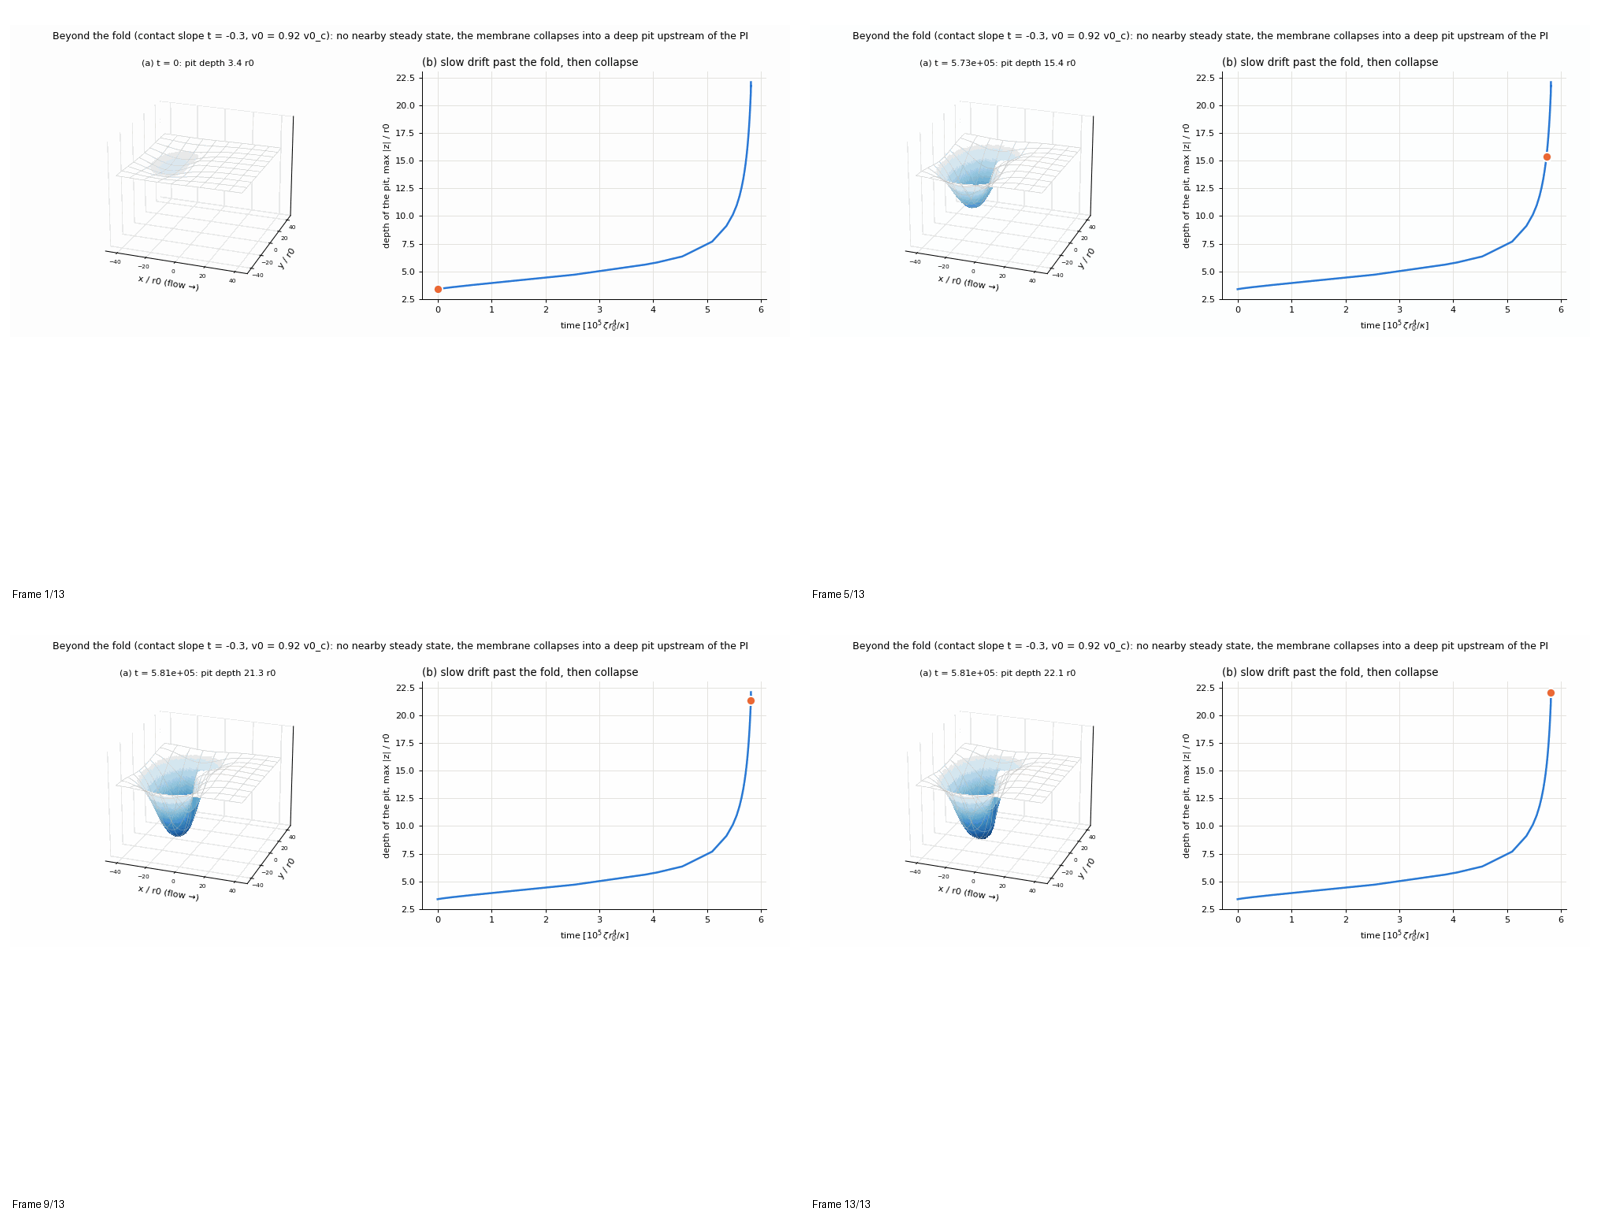
\includegraphics[width=\linewidth,height=170mm,keepaspectratio]{animation_stills/membrane_gif5_post_snap_collapse.png}\captionof{figure}[Archived figure]{Clamped-protein post-fold time integration: an upstream pit grows and the wall approaches vertical. Four ordered frames are selected by frame index; spacing is not asserted to be uniform in physical time. \textit{Original GIF:} \path{research/membrane_stability/figures/gifs/gif5_post_snap_collapse.gif}. First added 2026-10-01.}\end{center}
\noindent\textit{Playback file in this source package:} \path{figures/membrane_gif5_post_snap_collapse.gif}.\clearpage
\begin{center}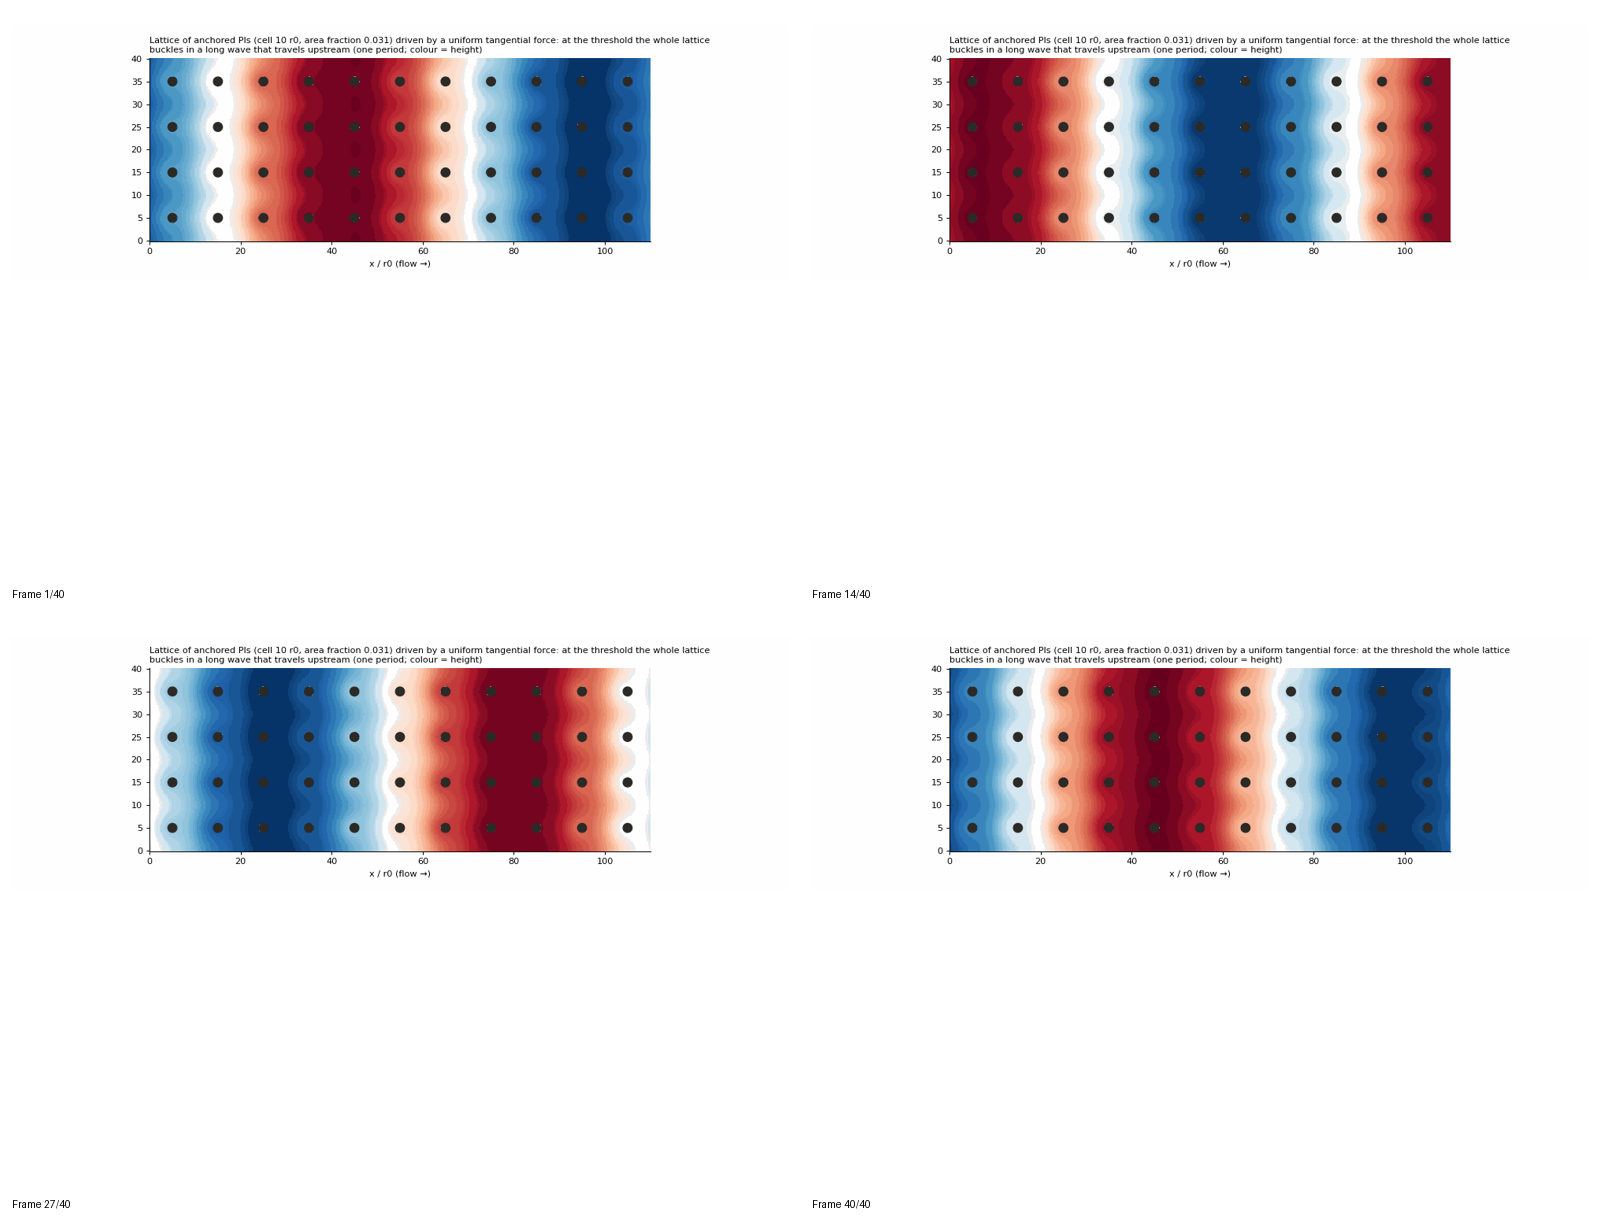
\includegraphics[width=\linewidth,height=170mm,keepaspectratio]{animation_stills/membrane_gif6_lattice_wave.png}\captionof{figure}[Archived figure]{Collective Bloch-wave pattern of a periodic protein array. This visualizes the long-wave instability and upstream phase drift, not a nonlinear terrace simulation. Four ordered frames are selected by frame index; spacing is not asserted to be uniform in physical time. \textit{Original GIF:} \path{research/membrane_stability/figures/gifs/gif6_lattice_wave.gif}. First added 2026-10-01.}\end{center}
\noindent\textit{Playback file in this source package:} \path{figures/membrane_gif6_lattice_wave.gif}.\clearpage
\begin{center}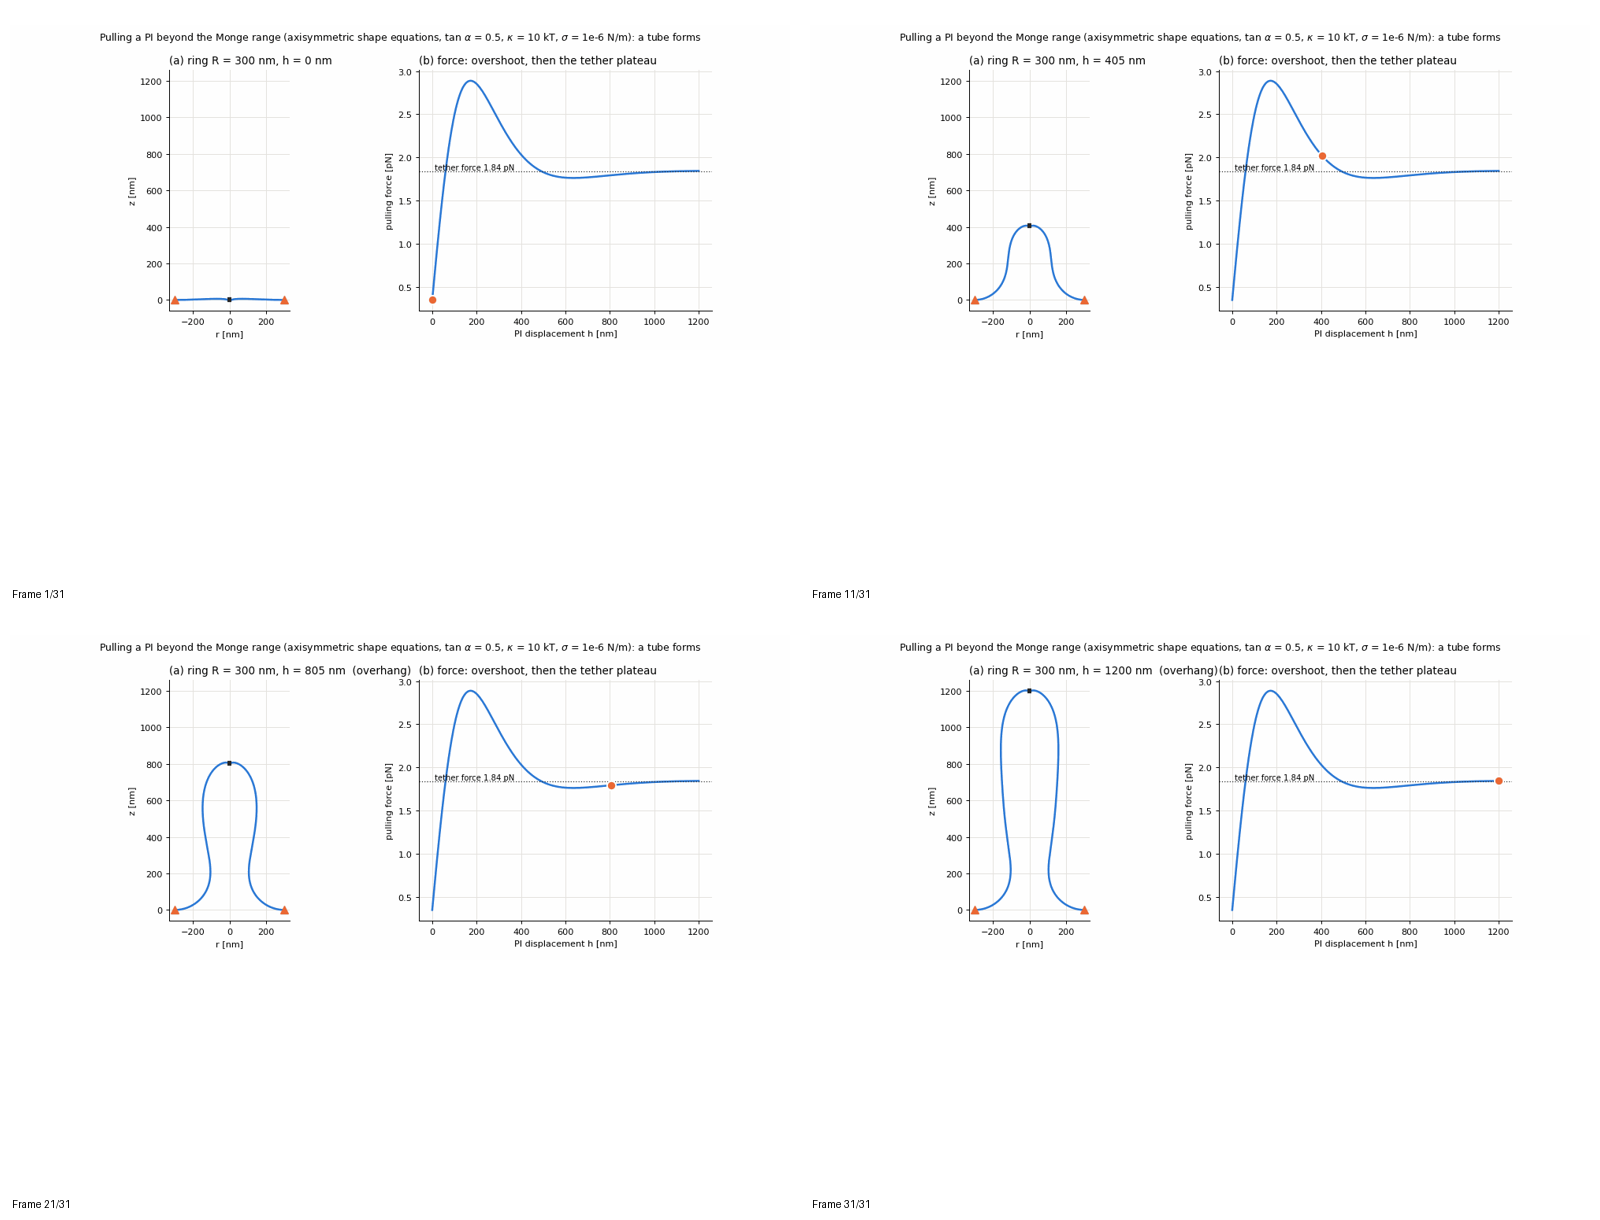
\includegraphics[width=\linewidth,height=170mm,keepaspectratio]{animation_stills/membrane_gif7_tube_extrusion.png}\captionof{figure}[Archived figure]{No-flow axisymmetric tube/neck continuation beyond the Monge range. The force plateau for a large ring agrees with tether theory. Four ordered frames are selected by frame index; spacing is not asserted to be uniform in physical time. \textit{Original GIF:} \path{research/membrane_stability/figures/gifs/gif7_tube_extrusion.gif}. First added 2026-10-01.}\end{center}
\noindent\textit{Playback file in this source package:} \path{figures/membrane_gif7_tube_extrusion.gif}.\clearpage
\begin{center}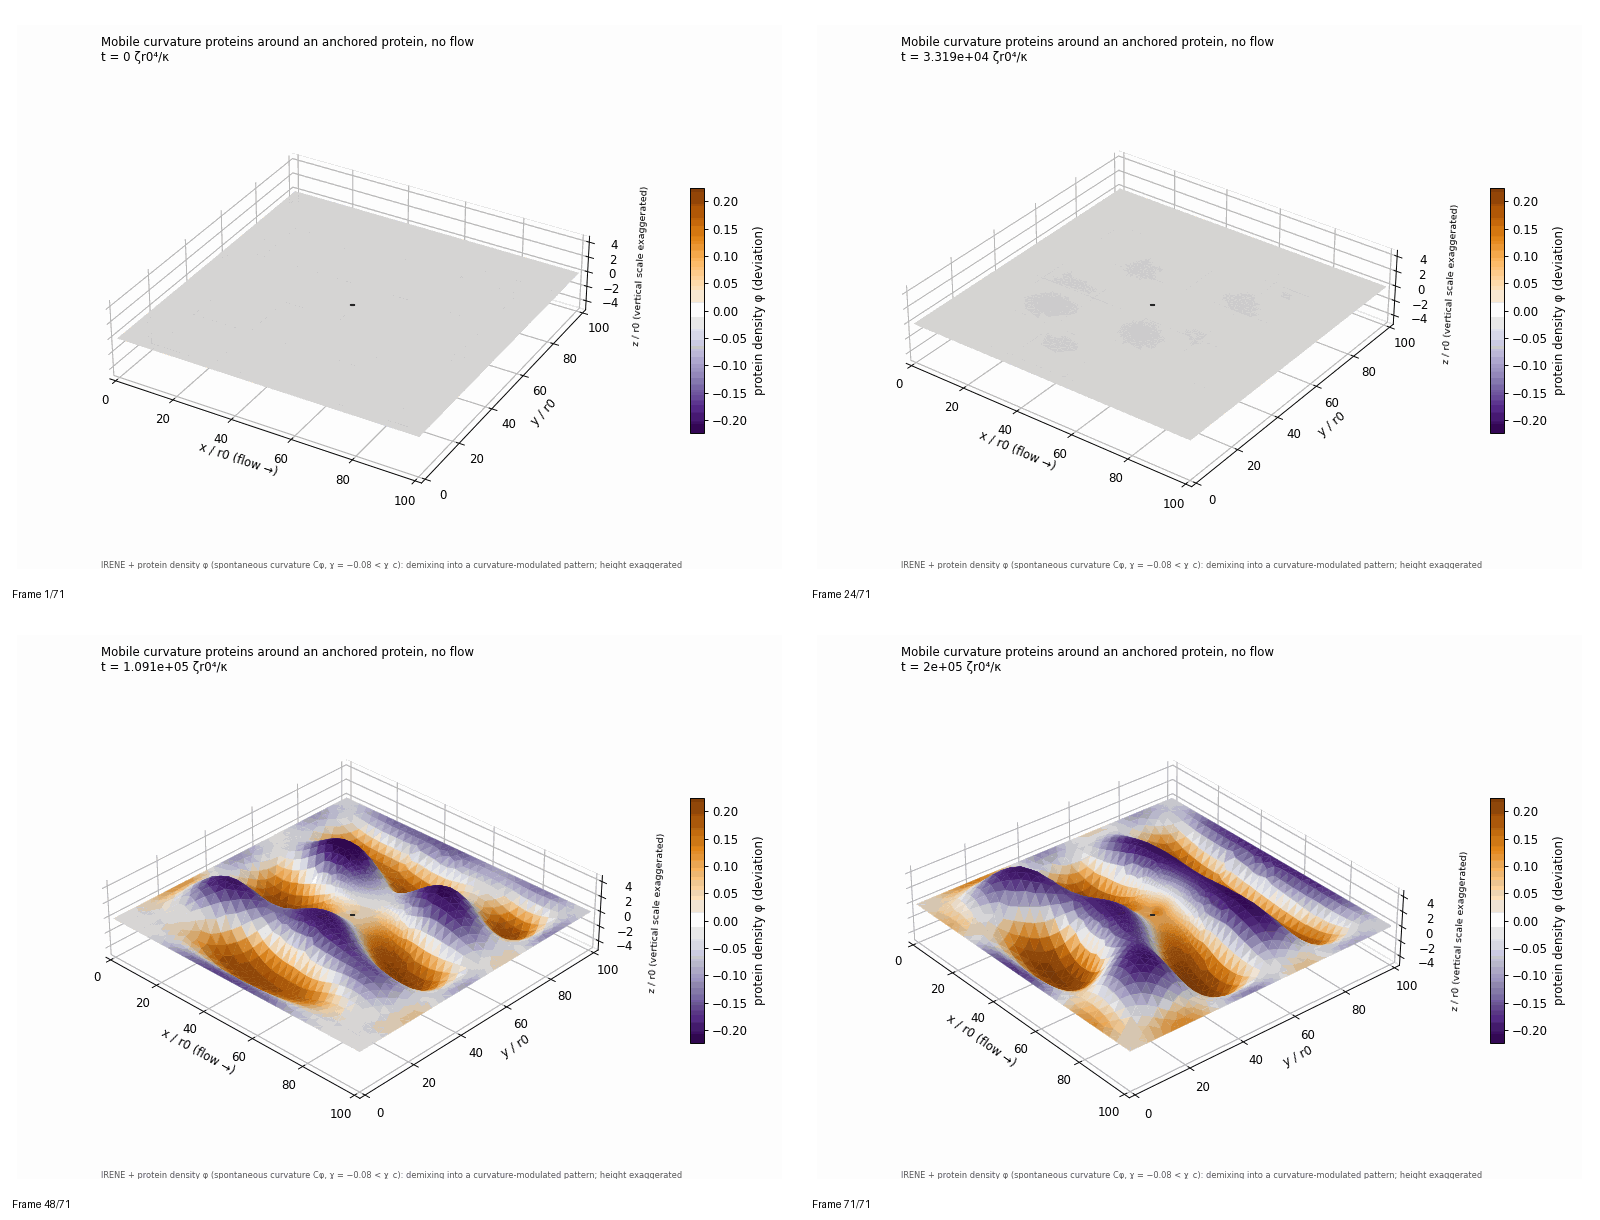
\includegraphics[width=\linewidth,height=170mm,keepaspectratio]{animation_stills/membrane_gif8_proteins_rest_3d.png}\captionof{figure}[Archived figure]{Consistent nonlinear curvature-protein demixing at rest. A modulated labyrinth forms while the free energy decreases. Four ordered frames are selected by frame index; spacing is not asserted to be uniform in physical time. \textit{Original GIF:} \path{research/membrane_stability/figures/gifs/gif8_proteins_rest_3d.gif}. First added 2026-10-02.}\end{center}
\noindent\textit{Playback file in this source package:} \path{figures/membrane_gif8_proteins_rest_3d.gif}.\clearpage
\begin{center}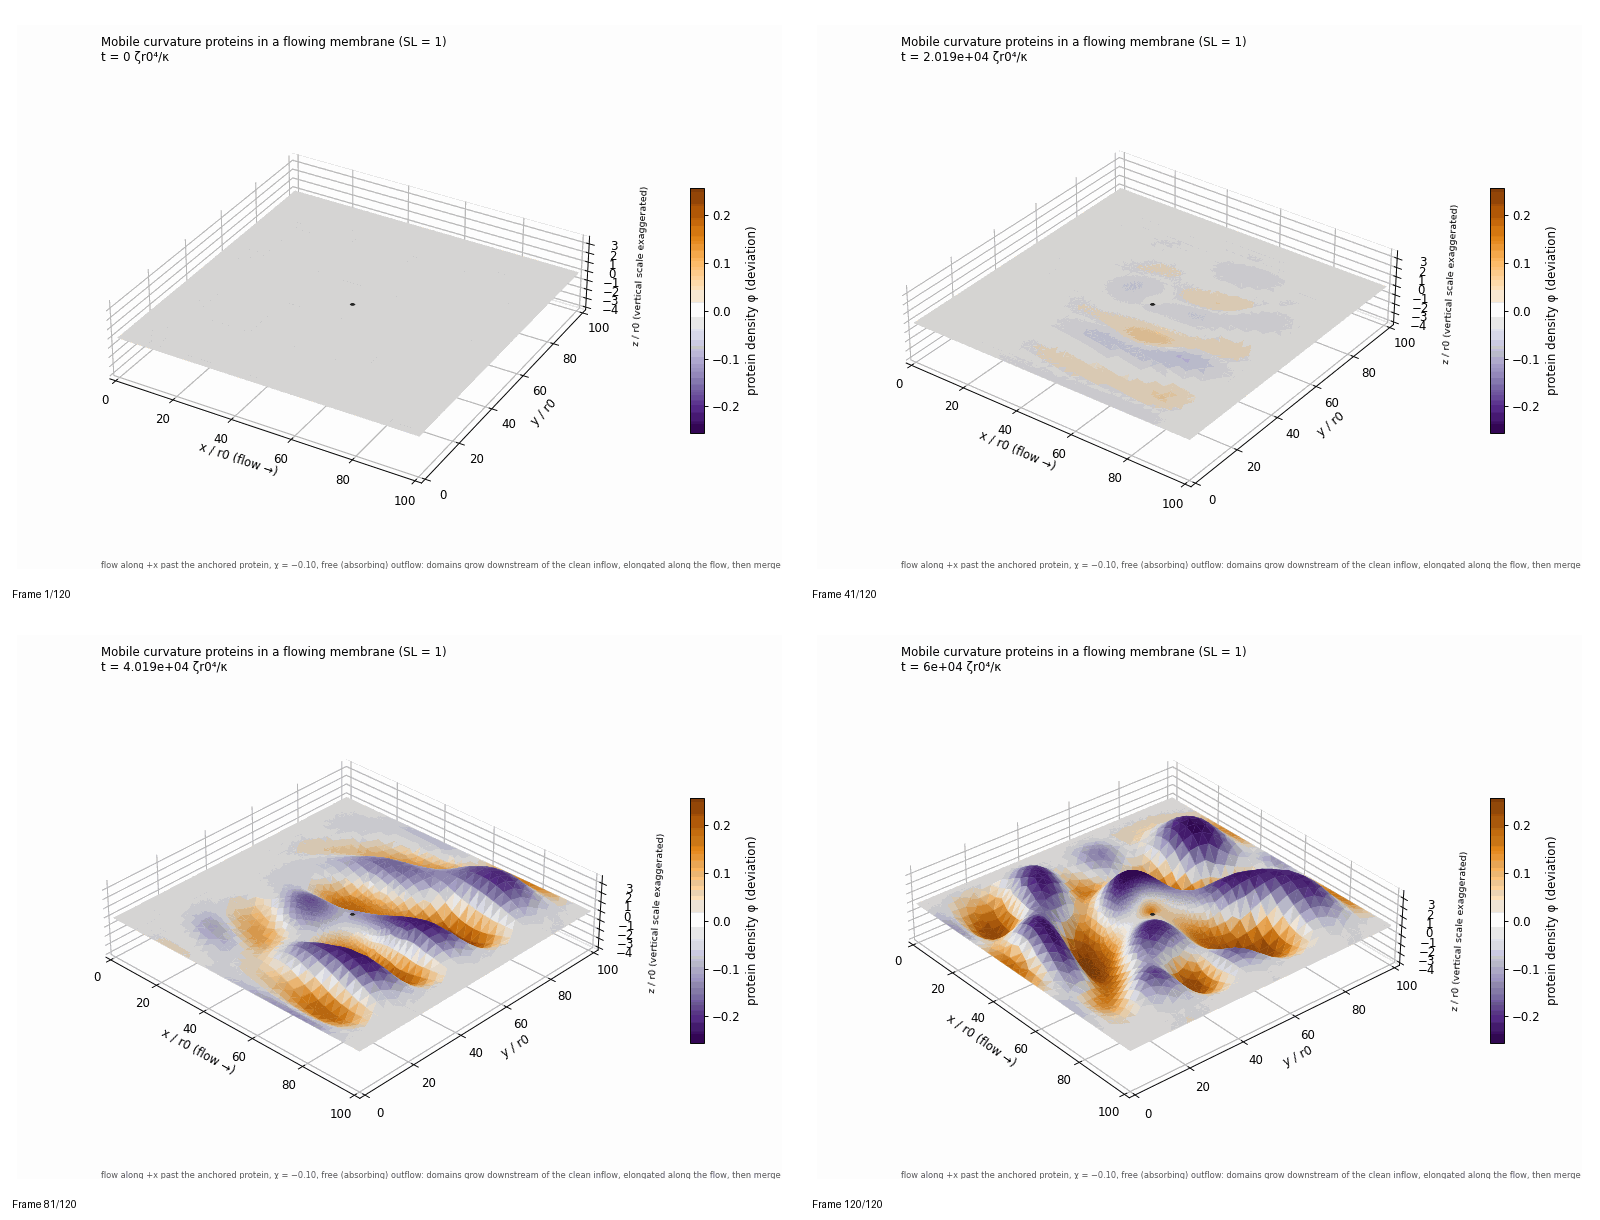
\includegraphics[width=\linewidth,height=170mm,keepaspectratio]{animation_stills/membrane_gif9_proteins_flow_3d.png}\captionof{figure}[Archived figure]{Mobile proteins in open flow. Downstream domains elongate along the flow and the membrane follows their curvature modulation. Four ordered frames are selected by frame index; spacing is not asserted to be uniform in physical time. \textit{Original GIF:} \path{research/membrane_stability/figures/gifs/gif9_proteins_flow_3d.gif}. First added 2026-10-02.}\end{center}
\noindent\textit{Playback file in this source package:} \path{figures/membrane_gif9_proteins_flow_3d.gif}.\clearpage
